% Options for packages loaded elsewhere
\PassOptionsToPackage{unicode}{hyperref}
\PassOptionsToPackage{hyphens}{url}
\PassOptionsToPackage{dvipsnames,svgnames,x11names}{xcolor}
%
\documentclass[
  letterpaper,
  DIV=11,
  numbers=noendperiod,
  abstract]{scrartcl}

\usepackage{amsmath,amssymb}
\usepackage{iftex}
\ifPDFTeX
  \usepackage[T1]{fontenc}
  \usepackage[utf8]{inputenc}
  \usepackage{textcomp} % provide euro and other symbols
\else % if luatex or xetex
  \usepackage{unicode-math}
  \defaultfontfeatures{Scale=MatchLowercase}
  \defaultfontfeatures[\rmfamily]{Ligatures=TeX,Scale=1}
\fi
\usepackage{lmodern}
\ifPDFTeX\else  
    % xetex/luatex font selection
\fi
% Use upquote if available, for straight quotes in verbatim environments
\IfFileExists{upquote.sty}{\usepackage{upquote}}{}
\IfFileExists{microtype.sty}{% use microtype if available
  \usepackage[]{microtype}
  \UseMicrotypeSet[protrusion]{basicmath} % disable protrusion for tt fonts
}{}
\makeatletter
\@ifundefined{KOMAClassName}{% if non-KOMA class
  \IfFileExists{parskip.sty}{%
    \usepackage{parskip}
  }{% else
    \setlength{\parindent}{0pt}
    \setlength{\parskip}{6pt plus 2pt minus 1pt}}
}{% if KOMA class
  \KOMAoptions{parskip=half}}
\makeatother
\usepackage{xcolor}
\setlength{\emergencystretch}{3em} % prevent overfull lines
\setcounter{secnumdepth}{5}
% Make \paragraph and \subparagraph free-standing
\ifx\paragraph\undefined\else
  \let\oldparagraph\paragraph
  \renewcommand{\paragraph}[1]{\oldparagraph{#1}\mbox{}}
\fi
\ifx\subparagraph\undefined\else
  \let\oldsubparagraph\subparagraph
  \renewcommand{\subparagraph}[1]{\oldsubparagraph{#1}\mbox{}}
\fi

\usepackage{color}
\usepackage{fancyvrb}
\newcommand{\VerbBar}{|}
\newcommand{\VERB}{\Verb[commandchars=\\\{\}]}
\DefineVerbatimEnvironment{Highlighting}{Verbatim}{commandchars=\\\{\}}
% Add ',fontsize=\small' for more characters per line
\usepackage{framed}
\definecolor{shadecolor}{RGB}{241,243,245}
\newenvironment{Shaded}{\begin{snugshade}}{\end{snugshade}}
\newcommand{\AlertTok}[1]{\textcolor[rgb]{0.68,0.00,0.00}{#1}}
\newcommand{\AnnotationTok}[1]{\textcolor[rgb]{0.37,0.37,0.37}{#1}}
\newcommand{\AttributeTok}[1]{\textcolor[rgb]{0.40,0.45,0.13}{#1}}
\newcommand{\BaseNTok}[1]{\textcolor[rgb]{0.68,0.00,0.00}{#1}}
\newcommand{\BuiltInTok}[1]{\textcolor[rgb]{0.00,0.23,0.31}{#1}}
\newcommand{\CharTok}[1]{\textcolor[rgb]{0.13,0.47,0.30}{#1}}
\newcommand{\CommentTok}[1]{\textcolor[rgb]{0.37,0.37,0.37}{#1}}
\newcommand{\CommentVarTok}[1]{\textcolor[rgb]{0.37,0.37,0.37}{\textit{#1}}}
\newcommand{\ConstantTok}[1]{\textcolor[rgb]{0.56,0.35,0.01}{#1}}
\newcommand{\ControlFlowTok}[1]{\textcolor[rgb]{0.00,0.23,0.31}{#1}}
\newcommand{\DataTypeTok}[1]{\textcolor[rgb]{0.68,0.00,0.00}{#1}}
\newcommand{\DecValTok}[1]{\textcolor[rgb]{0.68,0.00,0.00}{#1}}
\newcommand{\DocumentationTok}[1]{\textcolor[rgb]{0.37,0.37,0.37}{\textit{#1}}}
\newcommand{\ErrorTok}[1]{\textcolor[rgb]{0.68,0.00,0.00}{#1}}
\newcommand{\ExtensionTok}[1]{\textcolor[rgb]{0.00,0.23,0.31}{#1}}
\newcommand{\FloatTok}[1]{\textcolor[rgb]{0.68,0.00,0.00}{#1}}
\newcommand{\FunctionTok}[1]{\textcolor[rgb]{0.28,0.35,0.67}{#1}}
\newcommand{\ImportTok}[1]{\textcolor[rgb]{0.00,0.46,0.62}{#1}}
\newcommand{\InformationTok}[1]{\textcolor[rgb]{0.37,0.37,0.37}{#1}}
\newcommand{\KeywordTok}[1]{\textcolor[rgb]{0.00,0.23,0.31}{#1}}
\newcommand{\NormalTok}[1]{\textcolor[rgb]{0.00,0.23,0.31}{#1}}
\newcommand{\OperatorTok}[1]{\textcolor[rgb]{0.37,0.37,0.37}{#1}}
\newcommand{\OtherTok}[1]{\textcolor[rgb]{0.00,0.23,0.31}{#1}}
\newcommand{\PreprocessorTok}[1]{\textcolor[rgb]{0.68,0.00,0.00}{#1}}
\newcommand{\RegionMarkerTok}[1]{\textcolor[rgb]{0.00,0.23,0.31}{#1}}
\newcommand{\SpecialCharTok}[1]{\textcolor[rgb]{0.37,0.37,0.37}{#1}}
\newcommand{\SpecialStringTok}[1]{\textcolor[rgb]{0.13,0.47,0.30}{#1}}
\newcommand{\StringTok}[1]{\textcolor[rgb]{0.13,0.47,0.30}{#1}}
\newcommand{\VariableTok}[1]{\textcolor[rgb]{0.07,0.07,0.07}{#1}}
\newcommand{\VerbatimStringTok}[1]{\textcolor[rgb]{0.13,0.47,0.30}{#1}}
\newcommand{\WarningTok}[1]{\textcolor[rgb]{0.37,0.37,0.37}{\textit{#1}}}

\providecommand{\tightlist}{%
  \setlength{\itemsep}{0pt}\setlength{\parskip}{0pt}}\usepackage{longtable,booktabs,array}
\usepackage{calc} % for calculating minipage widths
% Correct order of tables after \paragraph or \subparagraph
\usepackage{etoolbox}
\makeatletter
\patchcmd\longtable{\par}{\if@noskipsec\mbox{}\fi\par}{}{}
\makeatother
% Allow footnotes in longtable head/foot
\IfFileExists{footnotehyper.sty}{\usepackage{footnotehyper}}{\usepackage{footnote}}
\makesavenoteenv{longtable}
\usepackage{graphicx}
\makeatletter
\def\maxwidth{\ifdim\Gin@nat@width>\linewidth\linewidth\else\Gin@nat@width\fi}
\def\maxheight{\ifdim\Gin@nat@height>\textheight\textheight\else\Gin@nat@height\fi}
\makeatother
% Scale images if necessary, so that they will not overflow the page
% margins by default, and it is still possible to overwrite the defaults
% using explicit options in \includegraphics[width, height, ...]{}
\setkeys{Gin}{width=\maxwidth,height=\maxheight,keepaspectratio}
% Set default figure placement to htbp
\makeatletter
\def\fps@figure{htbp}
\makeatother

\usepackage{booktabs}
\usepackage{caption}
\usepackage{longtable}
\usepackage{colortbl}
\usepackage{array}
\KOMAoption{captions}{tableheading}
\makeatletter
\makeatother
\makeatletter
\makeatother
\makeatletter
\@ifpackageloaded{caption}{}{\usepackage{caption}}
\AtBeginDocument{%
\ifdefined\contentsname
  \renewcommand*\contentsname{Table of contents}
\else
  \newcommand\contentsname{Table of contents}
\fi
\ifdefined\listfigurename
  \renewcommand*\listfigurename{List of Figures}
\else
  \newcommand\listfigurename{List of Figures}
\fi
\ifdefined\listtablename
  \renewcommand*\listtablename{List of Tables}
\else
  \newcommand\listtablename{List of Tables}
\fi
\ifdefined\figurename
  \renewcommand*\figurename{Figure}
\else
  \newcommand\figurename{Figure}
\fi
\ifdefined\tablename
  \renewcommand*\tablename{Table}
\else
  \newcommand\tablename{Table}
\fi
}
\@ifpackageloaded{float}{}{\usepackage{float}}
\floatstyle{ruled}
\@ifundefined{c@chapter}{\newfloat{codelisting}{h}{lop}}{\newfloat{codelisting}{h}{lop}[chapter]}
\floatname{codelisting}{Listing}
\newcommand*\listoflistings{\listof{codelisting}{List of Listings}}
\makeatother
\makeatletter
\@ifpackageloaded{caption}{}{\usepackage{caption}}
\@ifpackageloaded{subcaption}{}{\usepackage{subcaption}}
\makeatother
\makeatletter
\@ifpackageloaded{tcolorbox}{}{\usepackage[skins,breakable]{tcolorbox}}
\makeatother
\makeatletter
\@ifundefined{shadecolor}{\definecolor{shadecolor}{rgb}{.97, .97, .97}}
\makeatother
\makeatletter
\@ifundefined{codebgcolor}{\definecolor{codebgcolor}{HTML}{f8f8f8}}
\makeatother
\makeatletter
\makeatother
\ifLuaTeX
  \usepackage{selnolig}  % disable illegal ligatures
\fi
\usepackage[]{biblatex}
\addbibresource{references.bib}
\IfFileExists{bookmark.sty}{\usepackage{bookmark}}{\usepackage{hyperref}}
\IfFileExists{xurl.sty}{\usepackage{xurl}}{} % add URL line breaks if available
\urlstyle{same} % disable monospaced font for URLs
\hypersetup{
  pdftitle={Evaluation of 3D-var Data Assimilation of WRF Temperature Prediction Over Northwestern Türkiye: A Case Study for the Period of 11 and 16 August, 2004},
  pdfauthor={Mehmet AKSOY \& Sercan AKIL},
  colorlinks=true,
  linkcolor={blue},
  filecolor={Maroon},
  citecolor={Blue},
  urlcolor={Blue},
  pdfcreator={LaTeX via pandoc}}

\title{Evaluation of 3D-var Data Assimilation of WRF Temperature
Prediction Over Northwestern Türkiye: A Case Study for the Period of 11
and 16 August, 2004}
\author{Mehmet AKSOY \& Sercan AKIL}
\date{}

\begin{document}
\maketitle
\begin{abstract}
In this project, we have been evaluated temperature prediction of
assimilated and non assimilated WRF outputs over Northwestern Türkiye
for the period of 11-16 August, 2004. Observation of eleven temperature
gauges and corresponding WRF predictions in the study area have been
compared. Moreover, predictions were extracted from assimilated and non
assimilated raw WRF data of different domains with varied
spatio-temporal resolutions by using gauges coordinates. For this
purpose, visualization of results and calculation of error proceedings
were performed in R programming and Quarto publishing system.
\end{abstract}
\ifdefined\Shaded\renewenvironment{Shaded}{\begin{tcolorbox}[colback={codebgcolor}, boxrule=0pt, frame hidden, enhanced, breakable, borderline west={3pt}{0pt}{shadecolor}, sharp corners]}{\end{tcolorbox}}\fi

\renewcommand*\contentsname{Table of contents}
{
\hypersetup{linkcolor=}
\setcounter{tocdepth}{3}
\tableofcontents
}
\listoffigures
\listoftables
\hypertarget{introduction}{%
\section{Introduction}\label{introduction}}

\hypertarget{numerical-weather-prediction-nwp-models}{%
\subsection{Numerical Weather Prediction (NWP)
Models}\label{numerical-weather-prediction-nwp-models}}

Numerical Weather Prediction (NWP) models are used to predict weather
conditions by simulating the atmosphere, oceans, land surface and their
interactions. NWP models are based on mathematical equations
representing the physical behavior of the atmosphere. These equations
are translated into computer code and use governing equations, numerical
methods, parameterizations of other physical processes and combined with
initial and boundary conditions before running over a geographic area
(we call that geographic area as domain). These physical processes need
to be approximated in models because of huge simulation computer time
which is called as parameterization.

According to ECMWF report, \emph{these processes affect too a small area
to be predicted in full detail by NWP models. The major reason lies in
the limited computing power that still does not allow us to calculate
the all processes for any place on Earth} \autocite{frnda2022}.

\hypertarget{data-assimilation}{%
\subsection{Data Assimilation}\label{data-assimilation}}

NWP models start with an initial value and it is the challenge because
initial-value effects next predictions with an increasing error. Thus,
updating initial-value prediction is a method to improve prediction
accuracy which is called as data assimilation. Infrared radiance from
the geostationary satellites and on-site radiosonde observation data
assimilation are powerful tools to improve the weather forecast have
been widely applied with this purpose in the past a few decades
\autocite{geer2018}.

There are a number of data assimilation techniques used in weather
forecasting. One of the most prominent are the three and four
dimensional variational data assimilation methods (3D-var and 4D-var).
3D-var incorporates meteorological data only within a time window around
the initialization moment and in this method the analysis increment (an
increment is introduced due to the actual observations) does not evolve
in time, e.g.~it has effect only at the beginning of the simulation. On
the other hand 4D-var method uses tangent linear and adjoint models
which model the propagation of analysis increment and more computing
time is needed \autocite{vladimirov2020}.

\hypertarget{weather-research-and-forecasting-wrf-model}{%
\subsection{Weather Research and Forecasting (WRF)
model}\label{weather-research-and-forecasting-wrf-model}}

The Weather Research and Forecasting (WRF) model is a next-generation
open source mesoscale numerical weather prediction system. As it is open
source, it has a very flexible structure that allows it to be used by
met-offices, universities and atmospheric research centers
\autocite{powers2017}. The effort to develop WRF began in the latter
1990's and was a collaborative partnership of the National Center for
Atmospheric Research (NCAR), the National Oceanic and Atmospheric
Administration (NOAA), the U.S. Air Force, the Naval Research
Laboratory, the University of Oklahoma, and the Federal Aviation
Administration (\href{https://www.mmm.ucar.edu/models/wrf}{WRF web
page}).

The WRF model is used for operational weather forecasting and research
purposes at \emph{Turkish State Meteorological Service} since last two
decades, as it is at many meteorological services around the world. It
is the fact that data assimilation of observations into WRF model method
is very popular not only in Türkiye but also in all over world since it
has a great potential to improve model forecast skill by reducing errors
of initial conditions \autocite{yucel2014,yucel2015,bao2015,cheng2017}.

\hypertarget{operations-on-assimilated-wrf-data}{%
\section{Operations on Assimilated WRF
Data}\label{operations-on-assimilated-wrf-data}}

There are two files for two different domains as assimilated and
non-assimilated predictions of WRF model. Thus, there are four netcdf
files totally. We are going to define prediction variables, forecast
period and coverage of domains for each file.

\hypertarget{uploading-necessary-packages}{%
\subsection{Uploading Necessary
Packages}\label{uploading-necessary-packages}}

We will need several packages for some implementations in R, for
instance; opening of the netcdf files of WRF data, handling of WRF
outputs, visualization and similar operations
\autocite{readxl,tidyverse,ggplot2-2,ggpubr-2,raster,rnaturalearth,ncdf4,R.utils,sf,gt}.

\begin{Shaded}
\begin{Highlighting}[]
\FunctionTok{library}\NormalTok{(readxl)}
\FunctionTok{library}\NormalTok{(tidyverse)}
\FunctionTok{library}\NormalTok{(ggplot2)}
\FunctionTok{library}\NormalTok{(raster)}
\FunctionTok{library}\NormalTok{(rnaturalearth)}
\FunctionTok{library}\NormalTok{(ncdf4)}
\FunctionTok{library}\NormalTok{(R.utils)}
\FunctionTok{library}\NormalTok{(sf)}
\FunctionTok{library}\NormalTok{(gt)}
\FunctionTok{library}\NormalTok{(ggpubr)}
\end{Highlighting}
\end{Shaded}

\hypertarget{temperature-forecast-of-wrf-in-domain-1}{%
\subsection{Temperature Forecast of WRF in Domain
1}\label{temperature-forecast-of-wrf-in-domain-1}}

The code in the below reads a NetCDF file (fname) using the
\emph{nc\_open function} from the ncdf4 package. NetCDF is a file format
commonly used for storing multidimensional scientific data including NWP
model output.

Firstly, we opened the assimilated WRF output for domain 1. Using sink
function the content of WRF output at the attachments
(\href{https://github.com/maksoy88bjk/STAT_570_FINAL_PROJECT_MAKSOY-SAKIL/blob/main/aswout/wrfout_d01_2004-08-11_00_00_00.txt}{wrfout\_d01\_2004-08-11\_00\_00\_00.txt})
can be created. The data cover time and coverage domain information with
meteorological predictions such as potential temperature \textbf{(T)},
temperature at 2 meter \textbf{(T2)}, wind speed at ten meter
\textbf{(U10 \& V10)}, precipitation \textbf{(RAINC \& RAINNC)} and etc.
We need to use name of the variables to extract specific data variables
from the raw data.

\begin{Shaded}
\begin{Highlighting}[]
\NormalTok{fname }\OtherTok{\textless{}{-}} \FunctionTok{paste0}\NormalTok{(}\StringTok{"D:/Kitaplar/METU{-}PHD/Thesis/IsmailHocandanAldim\_Aksoy\_27092023/"}\NormalTok{,}
\StringTok{"aswout/wrfout\_d01\_2004{-}08{-}11\_00\_00\_00"}\NormalTok{)}
\NormalTok{nc\_data }\OtherTok{\textless{}{-}} \FunctionTok{nc\_open}\NormalTok{(fname)}

\NormalTok{\{}\FunctionTok{sink}\NormalTok{(}\FunctionTok{paste0}\NormalTok{(fname,}\StringTok{".txt"}\NormalTok{))}
  \FunctionTok{print}\NormalTok{(nc\_data)}
  \FunctionTok{sink}\NormalTok{()\}}
\end{Highlighting}
\end{Shaded}

In the WRF data, air temperature at 2 meter \emph{(the height of
observation at gauges)} is available. If 2 meter temperature is not
available in netcdf file, the calculation of
\href{http://gradsusr.org/pipermail/gradsusr/2011-December/031698.html}{Air
Temperature Prediction} from WRF data is described at the given link
based on
\href{https://www2.mmm.ucar.edu/wrf/users/docs/user_guide_v4/contents.html}{WRF
manual}. In such a case, \emph{perturbation potential temperature},
\emph{base pressure} and \emph{perturbation pressure} variables has to
be extracted to get air temperature prediction.

\begin{verbatim}
float T2[west_east,south_north,Time]   
    FieldType: 104
    MemoryOrder: XY 
    description: TEMP at 2 M
    units: K
    stagger: 
    coordinates: XLONG XLAT
\end{verbatim}

\hypertarget{spatial-resolution-domain-1}{%
\subsubsection{Spatial Resolution (Domain
1)}\label{spatial-resolution-domain-1}}

Spatial resolution of domain 1 is 12 km as you can see below \emph{(DX:
12000, DY:12000)}.

\begin{verbatim}
78 global attributes:
    TITLE:  OUTPUT FROM WRF V3.1.1 MODEL
    START_DATE: 2004-08-11_00:00:00
    SIMULATION_START_DATE: 2004-08-11_00:00:00
    WEST-EAST_GRID_DIMENSION: 192
    SOUTH-NORTH_GRID_DIMENSION: 116
    BOTTOM-TOP_GRID_DIMENSION: 28
    DX: 12000
    DY: 12000
\end{verbatim}

Here, the code extracts specific variables (longitude, latitude,
temperature, and time) from the NetCDF file using the \emph{ncvar\_get
function}.

There are \textbf{41} time steps which means we can get predictions
along the domain \textbf{(191x115)} for whole period. Additionally, the
data includes information for \textbf{27} layers from bottom to top of
the atmosphere. Fortunately, we do not have to deal with upper layers'
data since we just need to extract temperature predictions at 2 meters.

\begin{Shaded}
\begin{Highlighting}[]
\NormalTok{long}\OtherTok{\textless{}{-}} \FunctionTok{ncvar\_get}\NormalTok{(nc\_data, }\StringTok{"XLONG"}\NormalTok{)}
\NormalTok{lat}\OtherTok{\textless{}{-}} \FunctionTok{ncvar\_get}\NormalTok{(nc\_data, }\StringTok{"XLAT"}\NormalTok{, }\AttributeTok{verbose =}\NormalTok{ F)}

\NormalTok{temp}\OtherTok{\textless{}{-}} \FunctionTok{ncvar\_get}\NormalTok{(nc\_data, }\StringTok{"T2"}\NormalTok{) }
\FunctionTok{dim}\NormalTok{(temp)}
\end{Highlighting}
\end{Shaded}

\begin{verbatim}
[1] 191 115  41
\end{verbatim}

\begin{Shaded}
\begin{Highlighting}[]
\FunctionTok{dim}\NormalTok{(}\FunctionTok{ncvar\_get}\NormalTok{(nc\_data, }\StringTok{"T"}\NormalTok{))}
\end{Highlighting}
\end{Shaded}

\begin{verbatim}
[1] 191 115  27  41
\end{verbatim}

\hypertarget{forecast-period-time-interval-domain-1}{%
\subsubsection{Forecast Period \& Time Interval (Domain
1)}\label{forecast-period-time-interval-domain-1}}

We can also obtained the forecast horizon by getting time steps from the
data. After getting time steps, we see that forecast period is between
11 and 16 (00:00 UTC) August, 2004. In this case, the time interval for
the forecast period up to +120 hours \emph{(or five days)} is three
hour.

\begin{Shaded}
\begin{Highlighting}[]
\NormalTok{t }\OtherTok{\textless{}{-}} \FunctionTok{ncvar\_get}\NormalTok{(nc\_data, }\StringTok{"Times"}\NormalTok{); t}
\end{Highlighting}
\end{Shaded}

\begin{verbatim}
 [1] "2004-08-11_00:00:00" "2004-08-11_03:00:00" "2004-08-11_06:00:00"
 [4] "2004-08-11_09:00:00" "2004-08-11_12:00:00" "2004-08-11_15:00:00"
 [7] "2004-08-11_18:00:00" "2004-08-11_21:00:00" "2004-08-12_00:00:00"
[10] "2004-08-12_03:00:00" "2004-08-12_06:00:00" "2004-08-12_09:00:00"
[13] "2004-08-12_12:00:00" "2004-08-12_15:00:00" "2004-08-12_18:00:00"
[16] "2004-08-12_21:00:00" "2004-08-13_00:00:00" "2004-08-13_03:00:00"
[19] "2004-08-13_06:00:00" "2004-08-13_09:00:00" "2004-08-13_12:00:00"
[22] "2004-08-13_15:00:00" "2004-08-13_18:00:00" "2004-08-13_21:00:00"
[25] "2004-08-14_00:00:00" "2004-08-14_03:00:00" "2004-08-14_06:00:00"
[28] "2004-08-14_09:00:00" "2004-08-14_12:00:00" "2004-08-14_15:00:00"
[31] "2004-08-14_18:00:00" "2004-08-14_21:00:00" "2004-08-15_00:00:00"
[34] "2004-08-15_03:00:00" "2004-08-15_06:00:00" "2004-08-15_09:00:00"
[37] "2004-08-15_12:00:00" "2004-08-15_15:00:00" "2004-08-15_18:00:00"
[40] "2004-08-15_21:00:00" "2004-08-16_00:00:00"
\end{verbatim}

\begin{Shaded}
\begin{Highlighting}[]
\FunctionTok{ymd\_hms}\NormalTok{(t[}\DecValTok{41}\NormalTok{]) }\SpecialCharTok{{-}} \FunctionTok{ymd\_hms}\NormalTok{(t[}\DecValTok{1}\NormalTok{])}
\end{Highlighting}
\end{Shaded}

\begin{verbatim}
Time difference of 5 days
\end{verbatim}

\hypertarget{study-area-domain-1}{%
\subsubsection{Study Area (Domain 1)}\label{study-area-domain-1}}

Figure~\ref{fig-domain1} below shows the coverage of domain 1 where
covers Türkiye and its surrounding.

The code in the below creates a list of raster objects for each time
step from the extracted temperature from raw WRF data set. Kelvin unit
has been converted into Celcius by implementing -273.15. Raster objects
are used for working with gridded spatial data. Additionally,
\emph{ggplot2} package is used to create a map visualization. It
overlays the temperature data onto a map of countries, setting up
appropriate coordinate systems and color scales.

\begin{Shaded}
\begin{Highlighting}[]
\NormalTok{raster\_temp}\OtherTok{\textless{}{-}} \FunctionTok{list}\NormalTok{()}
\ControlFlowTok{for}\NormalTok{ (i }\ControlFlowTok{in} \DecValTok{1}\SpecialCharTok{:}\FunctionTok{dim}\NormalTok{(temp)[}\DecValTok{3}\NormalTok{])   \{}
\NormalTok{    raster\_temp[[i]] }\OtherTok{\textless{}{-}} \FunctionTok{raster}\NormalTok{(}\FunctionTok{t}\NormalTok{(temp[, , i] }\SpecialCharTok{{-}} \FloatTok{273.15}\NormalTok{), }
       \AttributeTok{xmn=}\FunctionTok{min}\NormalTok{(long), }\AttributeTok{xmx=}\FunctionTok{max}\NormalTok{(long),}
       \AttributeTok{ymn=}\FunctionTok{min}\NormalTok{(lat), }\AttributeTok{ymx=}\FunctionTok{max}\NormalTok{(lat), }
       \AttributeTok{crs=}\FunctionTok{CRS}\NormalTok{(}\StringTok{"+proj=longlat +ellps=WGS84 +datum=WGS84 +no\_defs+ towgs84=0,0,0"}\NormalTok{))}
\NormalTok{\}}

\NormalTok{temp\_df }\OtherTok{\textless{}{-}}\FunctionTok{as.data.frame}\NormalTok{(raster\_temp[[}\FunctionTok{length}\NormalTok{(t)]], }\AttributeTok{xy =} \ConstantTok{TRUE}\NormalTok{) }
\NormalTok{world }\OtherTok{\textless{}{-}}\NormalTok{ rnaturalearth}\SpecialCharTok{::}\FunctionTok{ne\_countries}\NormalTok{(}\AttributeTok{scale=}\StringTok{\textquotesingle{}medium\textquotesingle{}}\NormalTok{,}\AttributeTok{returnclass =} \StringTok{\textquotesingle{}sf\textquotesingle{}}\NormalTok{)}

\FunctionTok{ggplot}\NormalTok{(}\AttributeTok{data =}\NormalTok{ world)  }\SpecialCharTok{+} \FunctionTok{geom\_sf}\NormalTok{(}\AttributeTok{fill =} \StringTok{"white"}\NormalTok{) }\SpecialCharTok{+}
  \FunctionTok{coord\_sf}\NormalTok{(}\AttributeTok{crs =} \FunctionTok{st\_crs}\NormalTok{(}\DecValTok{4326}\NormalTok{), }\AttributeTok{xlim =} \FunctionTok{c}\NormalTok{(}\DecValTok{10}\NormalTok{, }\DecValTok{55}\NormalTok{), }\AttributeTok{ylim =} \FunctionTok{c}\NormalTok{(}\DecValTok{30}\NormalTok{,}\DecValTok{50}\NormalTok{)) }\SpecialCharTok{+}
  \FunctionTok{geom\_raster}\NormalTok{(}\AttributeTok{data =}\NormalTok{ temp\_df, }\FunctionTok{aes}\NormalTok{(x, y, }\AttributeTok{fill =}\NormalTok{ layer), }\AttributeTok{alpha=}\FloatTok{0.6}\NormalTok{) }\SpecialCharTok{+}
  \FunctionTok{scale\_fill\_viridis\_c}\NormalTok{(}\AttributeTok{limits =} \FunctionTok{c}\NormalTok{(}\DecValTok{0}\NormalTok{, }\DecValTok{35}\NormalTok{)) }\SpecialCharTok{+}
  \FunctionTok{labs}\NormalTok{(}\AttributeTok{x=}\StringTok{""}\NormalTok{,}\AttributeTok{y=}\StringTok{""}\NormalTok{, }\AttributeTok{fill=} \FunctionTok{expression}\NormalTok{(degree}\SpecialCharTok{*}\NormalTok{C)) }\SpecialCharTok{+} 
  \FunctionTok{ggtitle}\NormalTok{(}\StringTok{"Coverage of Domain 1"}\NormalTok{) }\SpecialCharTok{+} \FunctionTok{theme}\NormalTok{(}\AttributeTok{legend.key.height =} \FunctionTok{unit}\NormalTok{(}\DecValTok{1}\NormalTok{, }\StringTok{"cm"}\NormalTok{))}
\end{Highlighting}
\end{Shaded}

\begin{figure}[H]

{\centering 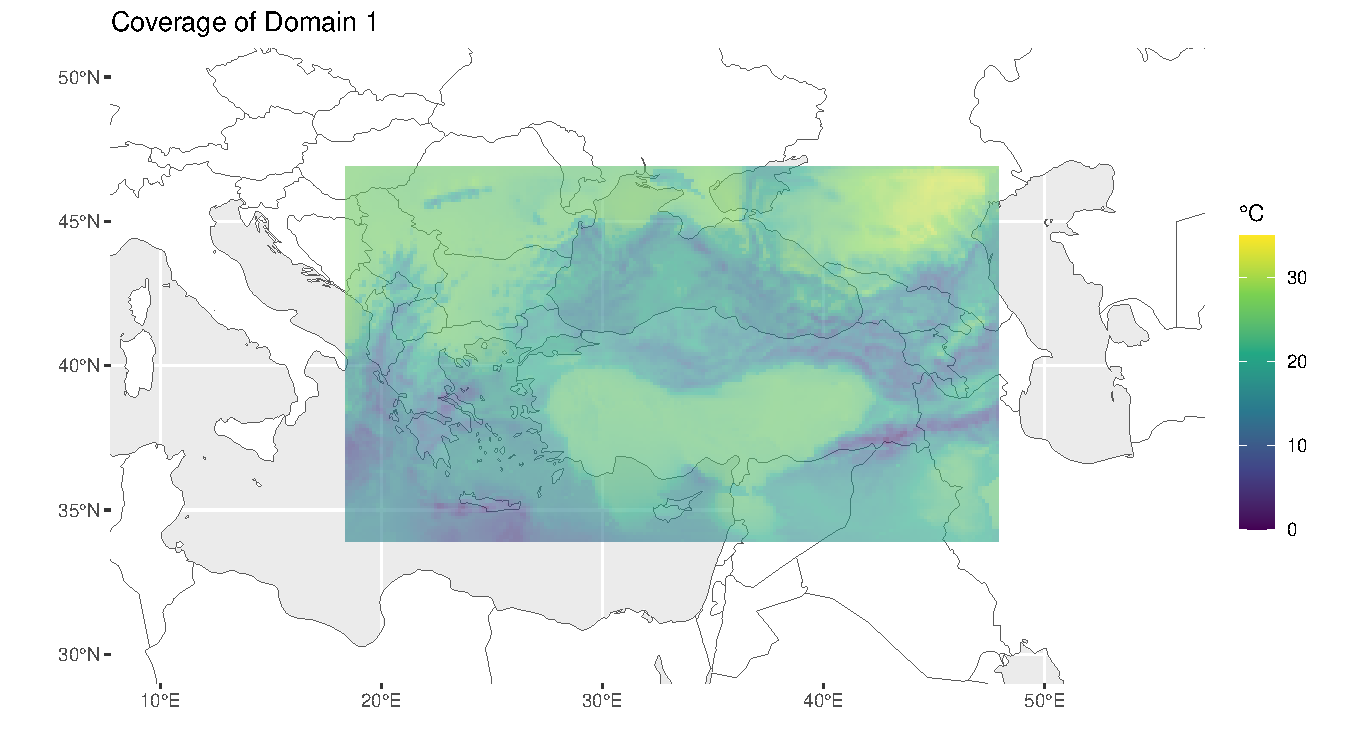
\includegraphics{WRF_pdf_files/figure-pdf/fig-domain1-1.pdf}

}

\caption{\label{fig-domain1}Türkiye with its neighboring countries and
coverage of domain 1 for assimilated-WRF predictions.}

\end{figure}

\hypertarget{temperature-forecast-of-wrf-in-domain-2}{%
\subsection{Temperature Forecast of WRF in Domain
2}\label{temperature-forecast-of-wrf-in-domain-2}}

There are \textbf{121} time steps for second domain since we can
inference by dimension of \textbf{T2} data.

\begin{Shaded}
\begin{Highlighting}[]
\NormalTok{fname2 }\OtherTok{\textless{}{-}} \FunctionTok{paste0}\NormalTok{(}\StringTok{"D:/Kitaplar/METU{-}PHD/Thesis/IsmailHocandanAldim\_Aksoy\_27092023/"}\NormalTok{,}
\StringTok{"aswout/wrfout\_d02\_2004{-}08{-}11\_00\_00\_00"}\NormalTok{)}
\NormalTok{nc\_data2 }\OtherTok{\textless{}{-}} \FunctionTok{nc\_open}\NormalTok{(fname2)}

\NormalTok{\{}\FunctionTok{sink}\NormalTok{(}\FunctionTok{paste0}\NormalTok{(fname2,}\StringTok{".txt"}\NormalTok{))}
  \FunctionTok{print}\NormalTok{(nc\_data2)}
  \FunctionTok{sink}\NormalTok{()\}}

\NormalTok{long\_2}\OtherTok{\textless{}{-}} \FunctionTok{ncvar\_get}\NormalTok{(nc\_data2, }\StringTok{"XLONG"}\NormalTok{)}
\NormalTok{lat\_2}\OtherTok{\textless{}{-}} \FunctionTok{ncvar\_get}\NormalTok{(nc\_data2, }\StringTok{"XLAT"}\NormalTok{, }\AttributeTok{verbose =}\NormalTok{ F)}
\NormalTok{temp\_2}\OtherTok{\textless{}{-}} \FunctionTok{ncvar\_get}\NormalTok{(nc\_data2, }\StringTok{"T2"}\NormalTok{) }

\FunctionTok{dim}\NormalTok{(temp\_2)}
\end{Highlighting}
\end{Shaded}

\begin{verbatim}
[1] 132  63 121
\end{verbatim}

\hypertarget{spatial-resolution-domain-2}{%
\subsubsection{Spatial Resolution (Domain
2)}\label{spatial-resolution-domain-2}}

Spatial resolution of domain 2 is 4 km which is a finer resolution than
previous one \emph{(DX: 4000, DY: 4000)}.

\begin{verbatim}
78 global attributes:
    TITLE:  OUTPUT FROM WRF V3.1.1 MODEL
    START_DATE: 2004-08-11_00:00:00
    SIMULATION_START_DATE: 2004-08-11_00:00:00
    WEST-EAST_GRID_DIMENSION: 133
    SOUTH-NORTH_GRID_DIMENSION: 64
    BOTTOM-TOP_GRID_DIMENSION: 28
    DX: 4000
    DY: 4000
\end{verbatim}

\hypertarget{forecast-period-time-interval-domain-2}{%
\subsubsection{Forecast Period \& Time Interval (Domain
2)}\label{forecast-period-time-interval-domain-2}}

Forecast period for domain 2 is same with previous one. However, the
time interval is one hour and it has a finer temporal resolution.

\begin{Shaded}
\begin{Highlighting}[]
\NormalTok{t2 }\OtherTok{\textless{}{-}} \FunctionTok{ncvar\_get}\NormalTok{(nc\_data2, }\StringTok{"Times"}\NormalTok{); t2}
\end{Highlighting}
\end{Shaded}

\begin{verbatim}
  [1] "2004-08-11_00:00:00" "2004-08-11_01:00:00" "2004-08-11_02:00:00"
  [4] "2004-08-11_03:00:00" "2004-08-11_04:00:00" "2004-08-11_05:00:00"
  [7] "2004-08-11_06:00:00" "2004-08-11_07:00:00" "2004-08-11_08:00:00"
 [10] "2004-08-11_09:00:00" "2004-08-11_10:00:00" "2004-08-11_11:00:00"
 [13] "2004-08-11_12:00:00" "2004-08-11_13:00:00" "2004-08-11_14:00:00"
 [16] "2004-08-11_15:00:00" "2004-08-11_16:00:00" "2004-08-11_17:00:00"
 [19] "2004-08-11_18:00:00" "2004-08-11_19:00:00" "2004-08-11_20:00:00"
 [22] "2004-08-11_21:00:00" "2004-08-11_22:00:00" "2004-08-11_23:00:00"
 [25] "2004-08-12_00:00:00" "2004-08-12_01:00:00" "2004-08-12_02:00:00"
 [28] "2004-08-12_03:00:00" "2004-08-12_04:00:00" "2004-08-12_05:00:00"
 [31] "2004-08-12_06:00:00" "2004-08-12_07:00:00" "2004-08-12_08:00:00"
 [34] "2004-08-12_09:00:00" "2004-08-12_10:00:00" "2004-08-12_11:00:00"
 [37] "2004-08-12_12:00:00" "2004-08-12_13:00:00" "2004-08-12_14:00:00"
 [40] "2004-08-12_15:00:00" "2004-08-12_16:00:00" "2004-08-12_17:00:00"
 [43] "2004-08-12_18:00:00" "2004-08-12_19:00:00" "2004-08-12_20:00:00"
 [46] "2004-08-12_21:00:00" "2004-08-12_22:00:00" "2004-08-12_23:00:00"
 [49] "2004-08-13_00:00:00" "2004-08-13_01:00:00" "2004-08-13_02:00:00"
 [52] "2004-08-13_03:00:00" "2004-08-13_04:00:00" "2004-08-13_05:00:00"
 [55] "2004-08-13_06:00:00" "2004-08-13_07:00:00" "2004-08-13_08:00:00"
 [58] "2004-08-13_09:00:00" "2004-08-13_10:00:00" "2004-08-13_11:00:00"
 [61] "2004-08-13_12:00:00" "2004-08-13_13:00:00" "2004-08-13_14:00:00"
 [64] "2004-08-13_15:00:00" "2004-08-13_16:00:00" "2004-08-13_17:00:00"
 [67] "2004-08-13_18:00:00" "2004-08-13_19:00:00" "2004-08-13_20:00:00"
 [70] "2004-08-13_21:00:00" "2004-08-13_22:00:00" "2004-08-13_23:00:00"
 [73] "2004-08-14_00:00:00" "2004-08-14_01:00:00" "2004-08-14_02:00:00"
 [76] "2004-08-14_03:00:00" "2004-08-14_04:00:00" "2004-08-14_05:00:00"
 [79] "2004-08-14_06:00:00" "2004-08-14_07:00:00" "2004-08-14_08:00:00"
 [82] "2004-08-14_09:00:00" "2004-08-14_10:00:00" "2004-08-14_11:00:00"
 [85] "2004-08-14_12:00:00" "2004-08-14_13:00:00" "2004-08-14_14:00:00"
 [88] "2004-08-14_15:00:00" "2004-08-14_16:00:00" "2004-08-14_17:00:00"
 [91] "2004-08-14_18:00:00" "2004-08-14_19:00:00" "2004-08-14_20:00:00"
 [94] "2004-08-14_21:00:00" "2004-08-14_22:00:00" "2004-08-14_23:00:00"
 [97] "2004-08-15_00:00:00" "2004-08-15_01:00:00" "2004-08-15_02:00:00"
[100] "2004-08-15_03:00:00" "2004-08-15_04:00:00" "2004-08-15_05:00:00"
[103] "2004-08-15_06:00:00" "2004-08-15_07:00:00" "2004-08-15_08:00:00"
[106] "2004-08-15_09:00:00" "2004-08-15_10:00:00" "2004-08-15_11:00:00"
[109] "2004-08-15_12:00:00" "2004-08-15_13:00:00" "2004-08-15_14:00:00"
[112] "2004-08-15_15:00:00" "2004-08-15_16:00:00" "2004-08-15_17:00:00"
[115] "2004-08-15_18:00:00" "2004-08-15_19:00:00" "2004-08-15_20:00:00"
[118] "2004-08-15_21:00:00" "2004-08-15_22:00:00" "2004-08-15_23:00:00"
[121] "2004-08-16_00:00:00"
\end{verbatim}

\begin{Shaded}
\begin{Highlighting}[]
\FunctionTok{ymd\_hms}\NormalTok{(t2[}\DecValTok{121}\NormalTok{]) }\SpecialCharTok{{-}} \FunctionTok{ymd\_hms}\NormalTok{(t2[}\DecValTok{1}\NormalTok{])}
\end{Highlighting}
\end{Shaded}

\begin{verbatim}
Time difference of 5 days
\end{verbatim}

\hypertarget{study-area-domain-2}{%
\subsubsection{Study Area (Domain 2)}\label{study-area-domain-2}}

Figure~\ref{fig-domain2} below shows the comparison of two domains and
coverage of domain 2 where covers some part of northwest of Türkiye.

It is clearly seen that the intersection of domain 1 and 2 is the entire
domain 2. Thus, our study area become only the entire domain 2.

\begin{Shaded}
\begin{Highlighting}[]
\NormalTok{raster\_temp\_2}\OtherTok{\textless{}{-}} \FunctionTok{list}\NormalTok{()}
\ControlFlowTok{for}\NormalTok{ (i }\ControlFlowTok{in} \DecValTok{1}\SpecialCharTok{:}\FunctionTok{dim}\NormalTok{(temp\_2)[}\DecValTok{3}\NormalTok{])   \{}
\NormalTok{  raster\_temp\_2[[i]] }\OtherTok{\textless{}{-}} \FunctionTok{raster}\NormalTok{(}\FunctionTok{t}\NormalTok{(temp\_2[, , i] }\SpecialCharTok{{-}} \FloatTok{273.15}\NormalTok{), }
     \AttributeTok{xmn=}\FunctionTok{min}\NormalTok{(long\_2), }\AttributeTok{xmx=}\FunctionTok{max}\NormalTok{(long\_2),}
     \AttributeTok{ymn=}\FunctionTok{min}\NormalTok{(lat\_2), }\AttributeTok{ymx=}\FunctionTok{max}\NormalTok{(lat\_2), }
     \AttributeTok{crs=}\FunctionTok{CRS}\NormalTok{(}\StringTok{"+proj=longlat +ellps=WGS84 +datum=WGS84 +no\_defs+ towgs84=0,0,0"}\NormalTok{))}
\NormalTok{                              \}}

\NormalTok{temp\_df\_2 }\OtherTok{\textless{}{-}}\FunctionTok{as.data.frame}\NormalTok{(raster\_temp\_2[[}\FunctionTok{length}\NormalTok{(t2)]], }\AttributeTok{xy =} \ConstantTok{TRUE}\NormalTok{) }
\NormalTok{world }\OtherTok{\textless{}{-}}\NormalTok{ rnaturalearth}\SpecialCharTok{::}\FunctionTok{ne\_countries}\NormalTok{(}\AttributeTok{scale=}\StringTok{\textquotesingle{}medium\textquotesingle{}}\NormalTok{,}\AttributeTok{returnclass =} \StringTok{\textquotesingle{}sf\textquotesingle{}}\NormalTok{)}

\FunctionTok{ggplot}\NormalTok{(}\AttributeTok{data =}\NormalTok{ world)  }\SpecialCharTok{+} \FunctionTok{geom\_sf}\NormalTok{(}\AttributeTok{fill =} \StringTok{"white"}\NormalTok{) }\SpecialCharTok{+} 
  \FunctionTok{coord\_sf}\NormalTok{(}\AttributeTok{crs =} \FunctionTok{st\_crs}\NormalTok{(}\DecValTok{4326}\NormalTok{), }\AttributeTok{xlim =} \FunctionTok{c}\NormalTok{(}\DecValTok{19}\NormalTok{, }\FloatTok{47.5}\NormalTok{), }\AttributeTok{ylim =} \FunctionTok{c}\NormalTok{(}\FloatTok{33.5}\NormalTok{,}\DecValTok{47}\NormalTok{)) }\SpecialCharTok{+}
  \FunctionTok{geom\_raster}\NormalTok{(}\AttributeTok{data =}\NormalTok{ temp\_df, }
            \FunctionTok{aes}\NormalTok{(x, y, }\AttributeTok{fill=}\NormalTok{ layer), }\AttributeTok{alpha=}\FloatTok{0.3}\NormalTok{, }\AttributeTok{show.legend =} \ConstantTok{FALSE}\NormalTok{) }\SpecialCharTok{+} 
  \FunctionTok{geom\_raster}\NormalTok{(}\AttributeTok{data =}\NormalTok{ temp\_df\_2, }
            \FunctionTok{aes}\NormalTok{(x, y, }\AttributeTok{fill=}\NormalTok{ layer), }\AttributeTok{alpha=}\FloatTok{0.7}\NormalTok{, }\AttributeTok{show.legend =} \ConstantTok{FALSE}\NormalTok{) }\SpecialCharTok{+} 
  \FunctionTok{scale\_fill\_viridis\_c}\NormalTok{() }\SpecialCharTok{+} \FunctionTok{labs}\NormalTok{(}\AttributeTok{x=}\StringTok{""}\NormalTok{,}\AttributeTok{y=}\StringTok{""}\NormalTok{) }\SpecialCharTok{+} 
  \FunctionTok{ggtitle}\NormalTok{(}\StringTok{"Coverage of Domain 2"}\NormalTok{) }
\end{Highlighting}
\end{Shaded}

\begin{figure}[H]

{\centering 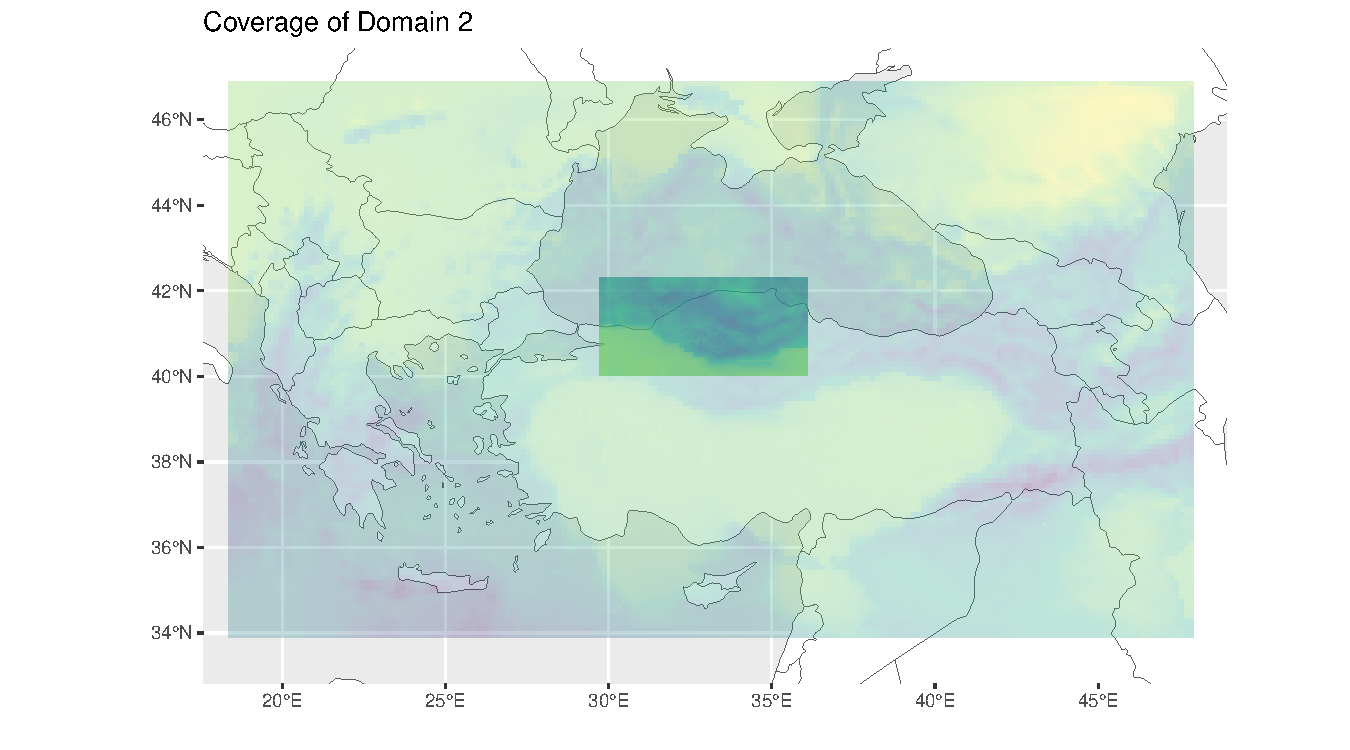
\includegraphics{WRF_pdf_files/figure-pdf/fig-domain2-1.pdf}

}

\caption{\label{fig-domain2}Comparison of domain 1 and 2.}

\end{figure}

\hypertarget{derivation-of-temperature-prediction-observation}{%
\subsection{Derivation of Temperature Prediction \&
Observation}\label{derivation-of-temperature-prediction-observation}}

\hypertarget{identification-of-meteorological-stations}{%
\subsubsection{Identification of Meteorological
Stations}\label{identification-of-meteorological-stations}}

Domain 2 covers several provinces which are located northwest of
Türkiye. Thus, we need to determine meteorological stations for
comparing observation versus assimilated and non-assimilated WRF
predictions. The code in the chunk reads data from a delimited text file
containing information about meteorological stations. Each specific
station was selected for each province to evaluate the performance of
both assimilated and non-assimilated WRF predictions.
Table~\ref{tbl-gauges-domain2} shows the main gauges across the domain
2.

The code uses the \emph{dplyr and gt} packages for data manipulation and
table creation. it assist to perform data wrangling and cleaning on the
meteorological station data, containing renaming columns, converting
province names, and arranging the data. The \emph{tolower function} is
used to convert the province names to lowercase. The
\emph{str\_to\_title() function} from the \emph{stringr} package is
applied to convert the province names' first letter to title case.

\begin{Shaded}
\begin{Highlighting}[]
\NormalTok{df\_gauges }\OtherTok{\textless{}{-}} \FunctionTok{read.delim}\NormalTok{(}\FunctionTok{paste0}\NormalTok{(}\StringTok{"D:/Kitaplar/METU{-}PHD/COURSES/3{-}TERM/"}\NormalTok{,}
\StringTok{"STAT\_570/STAT\_570\_FINAL\_PROJECT\_MAKSOY{-}SAKIL/gauges.txt"}\NormalTok{), }\AttributeTok{sep=}\StringTok{"|"}\NormalTok{)}

\NormalTok{df\_gauges}\OtherTok{\textless{}{-}}\NormalTok{ df\_gauges[,}\SpecialCharTok{{-}}\FunctionTok{c}\NormalTok{(}\DecValTok{3}\NormalTok{,}\DecValTok{4}\NormalTok{)]}
\FunctionTok{colnames}\NormalTok{(df\_gauges)}\OtherTok{\textless{}{-}} \FunctionTok{c}\NormalTok{(}\StringTok{"Station"}\NormalTok{,}\StringTok{"Province"}\NormalTok{,}\StringTok{"Latitude"}\NormalTok{,}\StringTok{"Longitude"}\NormalTok{,}\StringTok{"Altitude"}\NormalTok{) }

\NormalTok{df\_gauges}\SpecialCharTok{$}\NormalTok{Province }\OtherTok{\textless{}{-}} \FunctionTok{tolower}\NormalTok{(df\_gauges}\SpecialCharTok{$}\NormalTok{Province) }\SpecialCharTok{|\textgreater{}} \FunctionTok{str\_to\_title}\NormalTok{() }
\NormalTok{df\_gauges}\OtherTok{\textless{}{-}}\NormalTok{ df\_gauges }\SpecialCharTok{|\textgreater{}} \FunctionTok{arrange}\NormalTok{(Station) }
\NormalTok{df\_gauges }\SpecialCharTok{|\textgreater{}}  \FunctionTok{gt}\NormalTok{()}
\end{Highlighting}
\end{Shaded}

\hypertarget{tbl-gauges-domain2}{}
\begin{longtable}{rlrrr}
\caption{\label{tbl-gauges-domain2}Meteorological stations accross the domain 2. }\tabularnewline

\toprule
Station & Province & Latitude & Longitude & Altitude \\ 
\midrule\addlinespace[2.5pt]
17020 & Bartin & 41.62480 & 32.35690 & 33 \\ 
17022 & Zonguldak & 41.44924 & 31.77792 & 135 \\ 
17026 & Sinop & 42.02990 & 35.15450 & 32 \\ 
17069 & Sakarya & 40.76760 & 30.39340 & 30 \\ 
17070 & Bolu & 40.73290 & 31.60220 & 743 \\ 
17072 & Duzce & 40.84370 & 31.14880 & 146 \\ 
17074 & Kastamonu & 41.37100 & 33.77560 & 800 \\ 
17080 & Cankiri & 40.60820 & 33.61020 & 755 \\ 
17084 & Corum & 40.54610 & 34.93620 & 776 \\ 
17085 & Amasya & 40.66680 & 35.83530 & 409 \\ 
17622 & Samsun & 41.55150 & 35.92470 & 103 \\ 
\bottomrule
\end{longtable}

Figure~\ref{fig-gauges} is shown for distribution of meteorological
stations across the study area.

\begin{Shaded}
\begin{Highlighting}[]
\NormalTok{extents}\OtherTok{\textless{}{-}} \FunctionTok{extent}\NormalTok{(raster\_temp\_2[[}\FunctionTok{length}\NormalTok{(t2)]])}

\FunctionTok{ggplot}\NormalTok{(}\AttributeTok{data =}\NormalTok{ world)  }\SpecialCharTok{+} \FunctionTok{geom\_sf}\NormalTok{(}\AttributeTok{fill =} \StringTok{"white"}\NormalTok{) }\SpecialCharTok{+} 
  \FunctionTok{coord\_sf}\NormalTok{(}\AttributeTok{crs =} \FunctionTok{st\_crs}\NormalTok{(}\DecValTok{4326}\NormalTok{), }\AttributeTok{xlim =} \FunctionTok{c}\NormalTok{(extents[}\DecValTok{1}\NormalTok{], extents[}\DecValTok{2}\NormalTok{]), }
                               \AttributeTok{ylim =} \FunctionTok{c}\NormalTok{(extents[}\DecValTok{3}\NormalTok{],extents[}\DecValTok{4}\NormalTok{])) }\SpecialCharTok{+}
  \FunctionTok{geom\_raster}\NormalTok{(}\AttributeTok{data =}\NormalTok{ temp\_df\_2, }
        \FunctionTok{aes}\NormalTok{(x, y, }\AttributeTok{fill =}\NormalTok{ layer), }\AttributeTok{alpha=}\FloatTok{0.6}\NormalTok{) }\SpecialCharTok{+}
  \FunctionTok{scale\_fill\_viridis\_c}\NormalTok{(}\AttributeTok{limits =} \FunctionTok{c}\NormalTok{(}\DecValTok{10}\NormalTok{, }\DecValTok{25}\NormalTok{)) }\SpecialCharTok{+} 
  \FunctionTok{labs}\NormalTok{(}\AttributeTok{x=}\StringTok{""}\NormalTok{,}\AttributeTok{y=}\StringTok{""}\NormalTok{, }\AttributeTok{fill=} \FunctionTok{expression}\NormalTok{(degree}\SpecialCharTok{*}\NormalTok{C)) }\SpecialCharTok{+}
  \FunctionTok{geom\_point}\NormalTok{(}\AttributeTok{data =}\NormalTok{ df\_gauges, }\FunctionTok{aes}\NormalTok{(}\AttributeTok{x=}\NormalTok{Longitude, }\AttributeTok{y=}\NormalTok{Latitude),}
             \AttributeTok{size=}\DecValTok{3}\NormalTok{, }\AttributeTok{colour=}\StringTok{"darkred"}\NormalTok{) }\SpecialCharTok{+} 
  \FunctionTok{geom\_text}\NormalTok{(}\AttributeTok{data=}\NormalTok{ df\_gauges, }\AttributeTok{mapping =} \FunctionTok{aes}\NormalTok{(}\AttributeTok{x=}\NormalTok{Longitude, }\AttributeTok{y=}\NormalTok{Latitude, }
                                           \AttributeTok{label=}\NormalTok{Province), }\AttributeTok{nudge\_y =} \SpecialCharTok{{-}}\FloatTok{0.1}\NormalTok{) }\SpecialCharTok{+} 
  \FunctionTok{ggtitle}\NormalTok{(}\FunctionTok{paste}\NormalTok{(}\StringTok{"Hourly Assimilated WRF Temperature Forecast,"}\NormalTok{, t2[}\DecValTok{121}\NormalTok{])) }\SpecialCharTok{+}
  \FunctionTok{theme}\NormalTok{(}\AttributeTok{legend.key.width=}\FunctionTok{unit}\NormalTok{(}\DecValTok{3}\NormalTok{,}\StringTok{"cm"}\NormalTok{), }\AttributeTok{legend.position=}\StringTok{"bottom"}\NormalTok{)}
\end{Highlighting}
\end{Shaded}

\begin{figure}[H]

{\centering 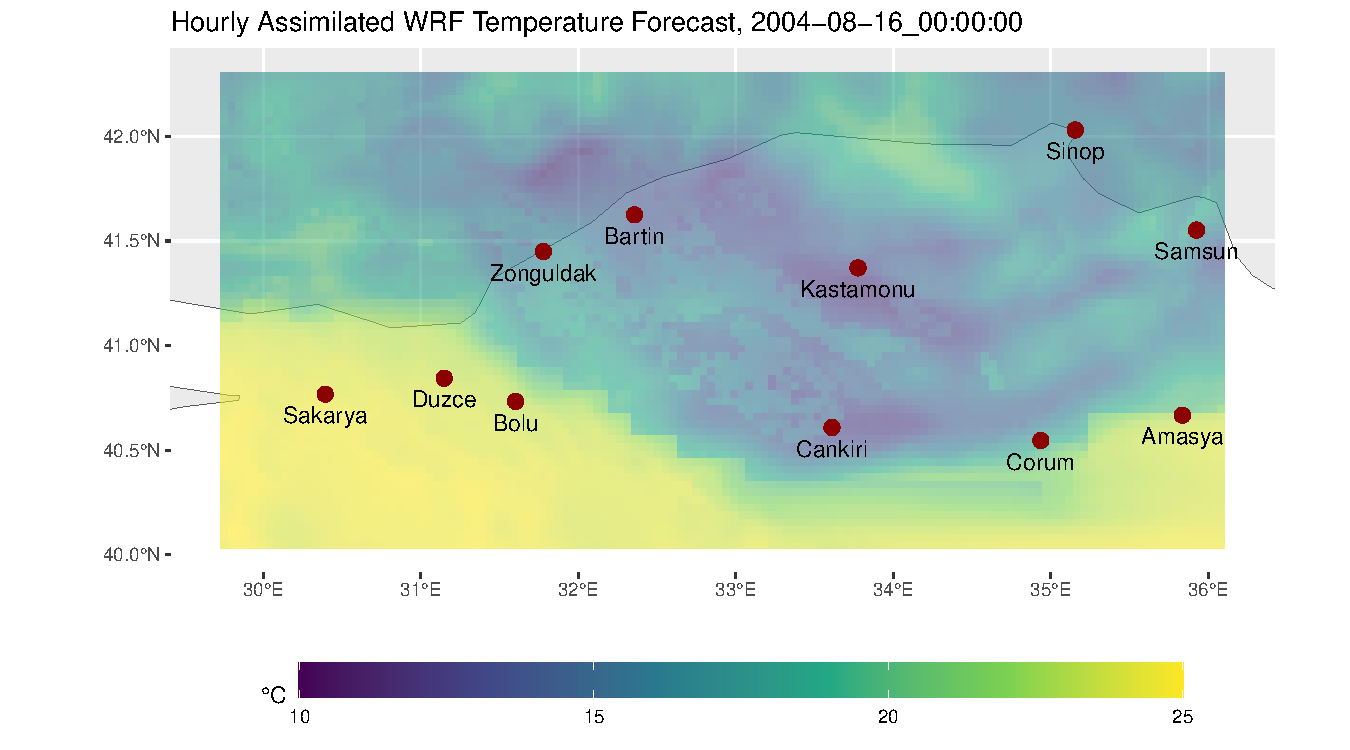
\includegraphics{WRF_pdf_files/figure-pdf/fig-gauges-1.pdf}

}

\caption{\label{fig-gauges}Distribution of Meteorological Stations Over
Domain 2.}

\end{figure}

\hypertarget{obtain-temperature-observations}{%
\subsubsection{Obtain Temperature
Observations}\label{obtain-temperature-observations}}

The code reads temperature observations from an excel file. In the raw
data, there is no date column but it has multiple columns which are
defined for year, month, day and hour information. Therefore, we need to
convert them into the single date column by merging them. Then, these
columns can be removed by non-selecting. In the raw data set, some dates
can be missing;however, these are not defined as null. Therefore,
leaping values can be detected then it assigned as a null by using
\emph{complete function}.

\begin{Shaded}
\begin{Highlighting}[]
\NormalTok{temp\_obs}\OtherTok{\textless{}{-}} \FunctionTok{read\_excel}\NormalTok{(}\FunctionTok{paste0}\NormalTok{(}\StringTok{"D:/Kitaplar/METU{-}PHD/COURSES/3{-}TERM/"}\NormalTok{,}
\StringTok{"STAT\_570/STAT\_570\_FINAL\_PROJECT\_MAKSOY{-}SAKIL/"}\NormalTok{,}
\StringTok{"df\_2023122096C0{-}Saatlik\_Sicaklik.xlsx"}\NormalTok{))}
\FunctionTok{head}\NormalTok{(temp\_obs)}
\end{Highlighting}
\end{Shaded}

\begin{verbatim}
# A tibble: 6 x 7
  Istasyon_No Istasyon_Adi   YIL    AY   GUN  SAAT SICAKLIK
        <dbl> <chr>        <dbl> <dbl> <dbl> <dbl>    <dbl>
1       17020 BARTIN        2004     8    10     0     18.7
2       17020 BARTIN        2004     8    10     1     18.3
3       17020 BARTIN        2004     8    10     2     18  
4       17020 BARTIN        2004     8    10     3     17.1
5       17020 BARTIN        2004     8    10     4     17.6
6       17020 BARTIN        2004     8    10     5     18.3
\end{verbatim}

\begin{Shaded}
\begin{Highlighting}[]
\NormalTok{temp\_obs}\OtherTok{\textless{}{-}}
\NormalTok{  temp\_obs }\SpecialCharTok{|\textgreater{}}
  \FunctionTok{mutate}\NormalTok{(}\AttributeTok{date=} \FunctionTok{as.Date}\NormalTok{(}\FunctionTok{with}\NormalTok{(temp\_obs, }\FunctionTok{paste}\NormalTok{(YIL,AY,GUN,}\AttributeTok{sep=}\StringTok{"{-}"}\NormalTok{)),}\StringTok{"\%Y{-}\%m{-}\%d"}\NormalTok{)) }\SpecialCharTok{|\textgreater{}}
  \FunctionTok{mutate}\NormalTok{(}\AttributeTok{dates=} \FunctionTok{ymd\_hms}\NormalTok{(}\FunctionTok{paste}\NormalTok{(date, }\FunctionTok{paste}\NormalTok{(SAAT, }\DecValTok{0}\NormalTok{, }\DecValTok{0}\NormalTok{, }\AttributeTok{sep =} \StringTok{":"}\NormalTok{)), }\AttributeTok{tz=}\StringTok{"UTC"}\NormalTok{)) }\SpecialCharTok{|\textgreater{}}
\NormalTok{  dplyr}\SpecialCharTok{::}\FunctionTok{select}\NormalTok{(Istasyon\_No, dates, SICAKLIK) }\SpecialCharTok{|\textgreater{}} 
  \FunctionTok{group\_by}\NormalTok{(Istasyon\_No) }\SpecialCharTok{|\textgreater{}} 
\NormalTok{  tidyr}\SpecialCharTok{::}\FunctionTok{complete}\NormalTok{( }\AttributeTok{dates =} \FunctionTok{seq}\NormalTok{(}\FunctionTok{ymd\_hm}\NormalTok{(}\StringTok{"2004{-}08{-}10 00:00"}\NormalTok{), }
                               \FunctionTok{ymd\_hm}\NormalTok{(}\StringTok{"2004{-}08{-}16 23:00"}\NormalTok{), }\AttributeTok{by =} \StringTok{"1 hours"}\NormalTok{))}

\FunctionTok{colnames}\NormalTok{(temp\_obs)}\OtherTok{\textless{}{-}} \FunctionTok{c}\NormalTok{(}\StringTok{"Station"}\NormalTok{,}\StringTok{"dates"}\NormalTok{,}\StringTok{"observation"}\NormalTok{)}
\FunctionTok{head}\NormalTok{(temp\_obs)}
\end{Highlighting}
\end{Shaded}

\begin{verbatim}
# A tibble: 6 x 3
# Groups:   Station [1]
  Station dates               observation
    <dbl> <dttm>                    <dbl>
1   17020 2004-08-10 00:00:00        18.7
2   17020 2004-08-10 01:00:00        18.3
3   17020 2004-08-10 02:00:00        18  
4   17020 2004-08-10 03:00:00        17.1
5   17020 2004-08-10 04:00:00        17.6
6   17020 2004-08-10 05:00:00        18.3
\end{verbatim}

\hypertarget{extraction-of-temperature-predictions-from-wrf}{%
\subsubsection{Extraction of Temperature Predictions from
WRF}\label{extraction-of-temperature-predictions-from-wrf}}

This code stacks raster layers (since time is not constant) and extracts
temperature values for meteorological station locations. Gauge locations
and prediction values with time need to be combined and data frame
columns need to be renamed after extraction procedure. The table below
contains three-hour temperature predictions for each province/gauge in
domain 1.

\begin{Shaded}
\begin{Highlighting}[]
\NormalTok{centroids }\OtherTok{\textless{}{-}}\NormalTok{ df\_gauges[,}\FunctionTok{c}\NormalTok{(}\DecValTok{1}\NormalTok{,}\DecValTok{3}\NormalTok{,}\DecValTok{4}\NormalTok{)]}
\FunctionTok{coordinates}\NormalTok{(centroids)}\OtherTok{=} \ErrorTok{\textasciitilde{}}\NormalTok{ Longitude }\SpecialCharTok{+}\NormalTok{ Latitude}

\CommentTok{\# domain1}
\NormalTok{raster\_temp\_stack}\OtherTok{\textless{}{-}} \FunctionTok{stack}\NormalTok{(raster\_temp)}
\NormalTok{raster\_temp\_value}\OtherTok{\textless{}{-}}\NormalTok{ raster}\SpecialCharTok{::}\FunctionTok{extract}\NormalTok{(raster\_temp\_stack, centroids)}

\NormalTok{rt\_cpv }\OtherTok{\textless{}{-}} \FunctionTok{cbind}\NormalTok{(centroids,raster\_temp\_value)}
\NormalTok{rt\_cpv\_df}\OtherTok{\textless{}{-}} \FunctionTok{data.frame}\NormalTok{(rt\_cpv)}
\FunctionTok{colnames}\NormalTok{(rt\_cpv\_df)}
\end{Highlighting}
\end{Shaded}

\begin{verbatim}
 [1] "Station"   "layer.1"   "layer.2"   "layer.3"   "layer.4"   "layer.5"  
 [7] "layer.6"   "layer.7"   "layer.8"   "layer.9"   "layer.10"  "layer.11" 
[13] "layer.12"  "layer.13"  "layer.14"  "layer.15"  "layer.16"  "layer.17" 
[19] "layer.18"  "layer.19"  "layer.20"  "layer.21"  "layer.22"  "layer.23" 
[25] "layer.24"  "layer.25"  "layer.26"  "layer.27"  "layer.28"  "layer.29" 
[31] "layer.30"  "layer.31"  "layer.32"  "layer.33"  "layer.34"  "layer.35" 
[37] "layer.36"  "layer.37"  "layer.38"  "layer.39"  "layer.40"  "layer.41" 
[43] "Longitude" "Latitude"  "optional" 
\end{verbatim}

\begin{Shaded}
\begin{Highlighting}[]
\NormalTok{rt\_cpv\_df}\OtherTok{\textless{}{-}}\NormalTok{ rt\_cpv\_df[,}\SpecialCharTok{{-}}\FunctionTok{ncol}\NormalTok{(rt\_cpv\_df)]}
\FunctionTok{head}\NormalTok{(rt\_cpv\_df)[,}\DecValTok{1}\SpecialCharTok{:}\DecValTok{5}\NormalTok{]}
\end{Highlighting}
\end{Shaded}

\begin{verbatim}
  Station  layer.1  layer.2  layer.3  layer.4
1   17020 19.14172 16.38781 18.63476 22.33074
2   17022 18.32778 17.36398 20.07202 23.92535
3   17026 20.14706 18.49960 20.52038 19.43371
4   17069 17.88046 15.75091 16.23025 19.67379
5   17070 16.78866 13.52252 16.43801 19.22317
6   17072 17.22476 14.45699 16.89929 19.99230
\end{verbatim}

\begin{Shaded}
\begin{Highlighting}[]
\NormalTok{rt\_cpv\_df}\OtherTok{\textless{}{-}} 
\NormalTok{  rt\_cpv\_df }\SpecialCharTok{|\textgreater{}} 
\NormalTok{  dplyr}\SpecialCharTok{::}\FunctionTok{select}\NormalTok{(Station, Longitude, Latitude,  }\FunctionTok{everything}\NormalTok{() )}
\FunctionTok{colnames}\NormalTok{(rt\_cpv\_df) }\OtherTok{\textless{}{-}} \FunctionTok{append}\NormalTok{(}\FunctionTok{colnames}\NormalTok{(rt\_cpv\_df[}\DecValTok{1}\SpecialCharTok{:}\DecValTok{3}\NormalTok{]),}\FunctionTok{as.character}\NormalTok{(t))}
\FunctionTok{head}\NormalTok{(rt\_cpv\_df)[,}\DecValTok{1}\SpecialCharTok{:}\DecValTok{5}\NormalTok{]}
\end{Highlighting}
\end{Shaded}

\begin{verbatim}
  Station Longitude Latitude 2004-08-11_00:00:00 2004-08-11_03:00:00
1   17020  32.35690 41.62480            19.14172            16.38781
2   17022  31.77792 41.44924            18.32778            17.36398
3   17026  35.15450 42.02990            20.14706            18.49960
4   17069  30.39340 40.76760            17.88046            15.75091
5   17070  31.60220 40.73290            16.78866            13.52252
6   17072  31.14880 40.84370            17.22476            14.45699
\end{verbatim}

Same procedures applied in previous chunk has to be followed for
assimilated data but for domain 2.

\begin{Shaded}
\begin{Highlighting}[]
\CommentTok{\# domain2}
\NormalTok{raster\_temp\_stack\_2}\OtherTok{\textless{}{-}} \FunctionTok{stack}\NormalTok{(raster\_temp\_2)}
\NormalTok{raster\_temp\_value\_2}\OtherTok{\textless{}{-}}\NormalTok{ raster}\SpecialCharTok{::}\FunctionTok{extract}\NormalTok{(raster\_temp\_stack\_2, centroids)}

\NormalTok{rt\_cpv\_2 }\OtherTok{\textless{}{-}} \FunctionTok{cbind}\NormalTok{(centroids,raster\_temp\_value\_2)}
\NormalTok{rt\_cpv\_df\_2}\OtherTok{\textless{}{-}} \FunctionTok{data.frame}\NormalTok{(rt\_cpv\_2) }
\NormalTok{rt\_cpv\_df\_2}\OtherTok{\textless{}{-}}\NormalTok{ rt\_cpv\_df\_2[,}\SpecialCharTok{{-}}\FunctionTok{ncol}\NormalTok{(rt\_cpv\_df\_2)]}

\NormalTok{rt\_cpv\_df\_2}\OtherTok{\textless{}{-}} 
\NormalTok{  rt\_cpv\_df\_2 }\SpecialCharTok{|\textgreater{}} 
\NormalTok{  dplyr}\SpecialCharTok{::}\FunctionTok{select}\NormalTok{(Station, Longitude, Latitude,  }\FunctionTok{everything}\NormalTok{() )}
\FunctionTok{colnames}\NormalTok{(rt\_cpv\_df\_2)}\OtherTok{\textless{}{-}} \FunctionTok{append}\NormalTok{(}\FunctionTok{colnames}\NormalTok{(rt\_cpv\_df\_2[}\DecValTok{1}\SpecialCharTok{:}\DecValTok{3}\NormalTok{]),}\FunctionTok{as.character}\NormalTok{(t2))}
\FunctionTok{head}\NormalTok{(rt\_cpv\_df\_2)[,}\DecValTok{1}\SpecialCharTok{:}\DecValTok{5}\NormalTok{]}
\end{Highlighting}
\end{Shaded}

\begin{verbatim}
  Station Longitude Latitude 2004-08-11_00:00:00 2004-08-11_01:00:00
1   17020  32.35690 41.62480            16.26486            12.88519
2   17022  31.77792 41.44924            16.93813            14.32098
3   17026  35.15450 42.02990            17.94399            18.06762
4   17069  30.39340 40.76760            20.76284            23.30419
5   17070  31.60220 40.73290            20.05142            22.39242
6   17072  31.14880 40.84370            20.31973            22.24160
\end{verbatim}

\hypertarget{operations-on-non-assimilated-wrf-data}{%
\section{Operations on Non-Assimilated WRF
Data}\label{operations-on-non-assimilated-wrf-data}}

We need to apply similar procedures on non-assimilated WRF predictions
for extraction as shown above.

\begin{Shaded}
\begin{Highlighting}[]
\CommentTok{\#domain1}
\NormalTok{fname\_nas }\OtherTok{\textless{}{-}} \FunctionTok{paste0}\NormalTok{(}\StringTok{"D:/Kitaplar/METU{-}PHD/Thesis/IsmailHocandanAldim\_Aksoy\_27092023/"}\NormalTok{,}
\StringTok{"wout/wrfout\_d01\_2004{-}08{-}11\_00\_00\_00"}\NormalTok{)}
\NormalTok{nc\_data\_nas }\OtherTok{\textless{}{-}} \FunctionTok{nc\_open}\NormalTok{(fname\_nas)}

\NormalTok{\{}\FunctionTok{sink}\NormalTok{(}\FunctionTok{paste0}\NormalTok{(fname\_nas,}\StringTok{".txt"}\NormalTok{))}
  \FunctionTok{print}\NormalTok{(nc\_data\_nas)}
  \FunctionTok{sink}\NormalTok{()\}}

\NormalTok{long\_nas}\OtherTok{\textless{}{-}} \FunctionTok{ncvar\_get}\NormalTok{(nc\_data\_nas, }\StringTok{"XLONG"}\NormalTok{)}
\NormalTok{lat\_nas}\OtherTok{\textless{}{-}} \FunctionTok{ncvar\_get}\NormalTok{(nc\_data\_nas, }\StringTok{"XLAT"}\NormalTok{, }\AttributeTok{verbose =}\NormalTok{ F)}
\NormalTok{temp\_nas}\OtherTok{\textless{}{-}} \FunctionTok{ncvar\_get}\NormalTok{(nc\_data\_nas, }\StringTok{"T2"}\NormalTok{) }
\NormalTok{t\_nas }\OtherTok{\textless{}{-}} \FunctionTok{ncvar\_get}\NormalTok{(nc\_data\_nas, }\StringTok{"Times"}\NormalTok{)}

\NormalTok{raster\_temp\_nas}\OtherTok{\textless{}{-}} \FunctionTok{list}\NormalTok{()}
\ControlFlowTok{for}\NormalTok{ (i }\ControlFlowTok{in} \DecValTok{1}\SpecialCharTok{:}\FunctionTok{dim}\NormalTok{(temp\_nas)[}\DecValTok{3}\NormalTok{])   \{}
\NormalTok{    raster\_temp\_nas[[i]] }\OtherTok{\textless{}{-}} \FunctionTok{raster}\NormalTok{(}\FunctionTok{t}\NormalTok{(temp\_nas[, , i] }\SpecialCharTok{{-}} \FloatTok{273.15}\NormalTok{), }
       \AttributeTok{xmn=}\FunctionTok{min}\NormalTok{(long\_nas), }\AttributeTok{xmx=}\FunctionTok{max}\NormalTok{(long\_nas),}
       \AttributeTok{ymn=}\FunctionTok{min}\NormalTok{(lat\_nas), }\AttributeTok{ymx=}\FunctionTok{max}\NormalTok{(lat\_nas), }
       \AttributeTok{crs=}\FunctionTok{CRS}\NormalTok{(}\StringTok{"+proj=longlat +ellps=WGS84 +datum=WGS84 +no\_defs+ towgs84=0,0,0"}\NormalTok{))}
\NormalTok{\}}

\CommentTok{\#domain2}
\NormalTok{fname2\_nas }\OtherTok{\textless{}{-}} \FunctionTok{paste0}\NormalTok{(}\StringTok{"D:/Kitaplar/METU{-}PHD/Thesis/IsmailHocandanAldim\_Aksoy\_27092023/"}\NormalTok{,}
\StringTok{"wout/wrfout\_d02\_2004{-}08{-}11\_00\_00\_00"}\NormalTok{)}
\NormalTok{nc\_data2\_nas }\OtherTok{\textless{}{-}} \FunctionTok{nc\_open}\NormalTok{(fname2\_nas)}

\NormalTok{\{}\FunctionTok{sink}\NormalTok{(}\FunctionTok{paste0}\NormalTok{(fname2\_nas,}\StringTok{".txt"}\NormalTok{))}
  \FunctionTok{print}\NormalTok{(nc\_data2\_nas)}
  \FunctionTok{sink}\NormalTok{()\}}

\NormalTok{long\_2\_nas}\OtherTok{\textless{}{-}} \FunctionTok{ncvar\_get}\NormalTok{(nc\_data2\_nas, }\StringTok{"XLONG"}\NormalTok{)}
\NormalTok{lat\_2\_nas}\OtherTok{\textless{}{-}} \FunctionTok{ncvar\_get}\NormalTok{(nc\_data2\_nas, }\StringTok{"XLAT"}\NormalTok{, }\AttributeTok{verbose =}\NormalTok{ F)}
\NormalTok{temp\_2\_nas}\OtherTok{\textless{}{-}} \FunctionTok{ncvar\_get}\NormalTok{(nc\_data2\_nas, }\StringTok{"T2"}\NormalTok{) }
\NormalTok{t2\_nas }\OtherTok{\textless{}{-}} \FunctionTok{ncvar\_get}\NormalTok{(nc\_data2\_nas, }\StringTok{"Times"}\NormalTok{)}

\NormalTok{raster\_temp\_2\_nas}\OtherTok{\textless{}{-}} \FunctionTok{list}\NormalTok{()}
\ControlFlowTok{for}\NormalTok{ (i }\ControlFlowTok{in} \DecValTok{1}\SpecialCharTok{:}\FunctionTok{dim}\NormalTok{(temp\_2\_nas)[}\DecValTok{3}\NormalTok{])   \{}
\NormalTok{    raster\_temp\_2\_nas[[i]] }\OtherTok{\textless{}{-}} \FunctionTok{raster}\NormalTok{(}\FunctionTok{t}\NormalTok{(temp\_2\_nas[, , i] }\SpecialCharTok{{-}} \FloatTok{273.15}\NormalTok{), }
       \AttributeTok{xmn=}\FunctionTok{min}\NormalTok{(long\_2\_nas), }\AttributeTok{xmx=}\FunctionTok{max}\NormalTok{(long\_2\_nas),}
       \AttributeTok{ymn=}\FunctionTok{min}\NormalTok{(lat\_2\_nas), }\AttributeTok{ymx=}\FunctionTok{max}\NormalTok{(lat\_2\_nas), }
       \AttributeTok{crs=}\FunctionTok{CRS}\NormalTok{(}\StringTok{"+proj=longlat +ellps=WGS84 +datum=WGS84 +no\_defs+ towgs84=0,0,0"}\NormalTok{))}
\NormalTok{\}}

\CommentTok{\# domain1}
\NormalTok{raster\_temp\_stack\_nas}\OtherTok{\textless{}{-}} \FunctionTok{stack}\NormalTok{(raster\_temp\_nas)}
\NormalTok{raster\_temp\_value\_nas}\OtherTok{\textless{}{-}}\NormalTok{ raster}\SpecialCharTok{::}\FunctionTok{extract}\NormalTok{(raster\_temp\_stack\_nas, centroids)}

\NormalTok{rt\_cpv\_nas }\OtherTok{\textless{}{-}} \FunctionTok{cbind}\NormalTok{(centroids,raster\_temp\_value\_nas)}
\NormalTok{rt\_cpv\_df\_nas}\OtherTok{\textless{}{-}} \FunctionTok{data.frame}\NormalTok{(rt\_cpv\_nas)}
\NormalTok{rt\_cpv\_df\_nas}\OtherTok{\textless{}{-}}\NormalTok{ rt\_cpv\_df\_nas[,}\SpecialCharTok{{-}}\FunctionTok{ncol}\NormalTok{(rt\_cpv\_df\_nas)]}

\NormalTok{rt\_cpv\_df\_nas}\OtherTok{\textless{}{-}} 
\NormalTok{  rt\_cpv\_df\_nas }\SpecialCharTok{|\textgreater{}} 
\NormalTok{  dplyr}\SpecialCharTok{::}\FunctionTok{select}\NormalTok{(Station, Longitude, Latitude,  }\FunctionTok{everything}\NormalTok{() )}
\FunctionTok{colnames}\NormalTok{(rt\_cpv\_df\_nas) }\OtherTok{\textless{}{-}} \FunctionTok{append}\NormalTok{(}\FunctionTok{colnames}\NormalTok{(rt\_cpv\_df\_nas[}\DecValTok{1}\SpecialCharTok{:}\DecValTok{3}\NormalTok{]),}\FunctionTok{as.character}\NormalTok{(t\_nas))}

\CommentTok{\# domain2}
\NormalTok{raster\_temp\_stack\_2\_nas}\OtherTok{\textless{}{-}} \FunctionTok{stack}\NormalTok{(raster\_temp\_2\_nas)}
\NormalTok{raster\_temp\_value\_2\_nas}\OtherTok{\textless{}{-}}\NormalTok{ raster}\SpecialCharTok{::}\FunctionTok{extract}\NormalTok{(raster\_temp\_stack\_2\_nas, centroids)}

\NormalTok{rt\_cpv\_2\_nas }\OtherTok{\textless{}{-}} \FunctionTok{cbind}\NormalTok{(centroids,raster\_temp\_value\_2\_nas)}
\NormalTok{rt\_cpv\_df\_2\_nas}\OtherTok{\textless{}{-}} \FunctionTok{data.frame}\NormalTok{(rt\_cpv\_2\_nas) }
\NormalTok{rt\_cpv\_df\_2\_nas}\OtherTok{\textless{}{-}}\NormalTok{ rt\_cpv\_df\_2\_nas[,}\SpecialCharTok{{-}}\FunctionTok{ncol}\NormalTok{(rt\_cpv\_df\_2\_nas)]}

\NormalTok{rt\_cpv\_df\_2\_nas}\OtherTok{\textless{}{-}} 
\NormalTok{  rt\_cpv\_df\_2\_nas }\SpecialCharTok{|\textgreater{}} 
\NormalTok{  dplyr}\SpecialCharTok{::}\FunctionTok{select}\NormalTok{(Station, Longitude, Latitude,  }\FunctionTok{everything}\NormalTok{() )}
\FunctionTok{colnames}\NormalTok{(rt\_cpv\_df\_2\_nas)}\OtherTok{\textless{}{-}} \FunctionTok{append}\NormalTok{(}\FunctionTok{colnames}\NormalTok{(rt\_cpv\_df\_2\_nas[}\DecValTok{1}\SpecialCharTok{:}\DecValTok{3}\NormalTok{]),}\FunctionTok{as.character}\NormalTok{(t2\_nas))}

\FunctionTok{head}\NormalTok{(rt\_cpv\_df\_2\_nas)[,}\DecValTok{1}\SpecialCharTok{:}\DecValTok{5}\NormalTok{]}
\end{Highlighting}
\end{Shaded}

\begin{verbatim}
  Station Longitude Latitude 2004-08-11_00:00:00 2004-08-11_01:00:00
1   17020  32.35690 41.62480            16.26486            12.82797
2   17022  31.77792 41.44924            16.93813            14.35607
3   17026  35.15450 42.02990            17.94399            17.90621
4   17069  30.39340 40.76760            20.76284            23.27804
5   17070  31.60220 40.73290            20.05142            22.38864
6   17072  31.14880 40.84370            20.31973            22.20229
\end{verbatim}

\hypertarget{results}{%
\section{Results}\label{results}}

\hypertarget{derivation-of-data-frames}{%
\subsection{Derivation of Data Frames}\label{derivation-of-data-frames}}

There are four data frames, including predictions and observations, to
represent each domain and assimilation version. However, these data
frames are wider format and it is needed to convert them longer since to
use them in visualization.

\begin{Shaded}
\begin{Highlighting}[]
\CommentTok{\# domain1 assimilated prediction: rt\_cpv\_df}
\CommentTok{\# domain2 assimilated prediction: rt\_cpv\_df\_2}

\CommentTok{\# domain1 non\_assimilated prediction: rt\_cpv\_df\_nas}
\CommentTok{\# domain2 non\_assimilated prediction: rt\_cpv\_df\_2\_nas}

\CommentTok{\# observations: temp\_obs}

\NormalTok{data\_list}\OtherTok{\textless{}{-}} \FunctionTok{list}\NormalTok{(rt\_cpv\_df, rt\_cpv\_df\_2, rt\_cpv\_df\_nas, rt\_cpv\_df\_2\_nas)}
\NormalTok{new\_df\_list}\OtherTok{\textless{}{-}} \FunctionTok{list}\NormalTok{()}
\NormalTok{variable}\OtherTok{\textless{}{-}} \FunctionTok{c}\NormalTok{(}\StringTok{"predict\_do1"}\NormalTok{, }\StringTok{"predict\_do2"}\NormalTok{,}\StringTok{"predict\_do1\_nas"}\NormalTok{,}\StringTok{"predict\_do2\_nas"}\NormalTok{)}
  
\ControlFlowTok{for}\NormalTok{(i }\ControlFlowTok{in} \DecValTok{1}\SpecialCharTok{:}\FunctionTok{length}\NormalTok{(variable))\{}
\NormalTok{  new\_df\_list[[i]] }\OtherTok{\textless{}{-}} 
\NormalTok{        data\_list[[i]] }\SpecialCharTok{|\textgreater{}} 
        \FunctionTok{distinct}\NormalTok{(Station, }\AttributeTok{.keep\_all =} \ConstantTok{TRUE}\NormalTok{) }\SpecialCharTok{|\textgreater{}} 
        \FunctionTok{pivot\_longer}\NormalTok{(}
          \AttributeTok{cols =} \FunctionTok{starts\_with}\NormalTok{(}\StringTok{"2004"}\NormalTok{),}
          \AttributeTok{names\_to =} \StringTok{"dates"}\NormalTok{,}
          \AttributeTok{values\_to =}\NormalTok{ variable[i],}
          \AttributeTok{values\_drop\_na =} \ConstantTok{FALSE}
\NormalTok{        ) }\SpecialCharTok{|\textgreater{}} 
\NormalTok{        dplyr}\SpecialCharTok{::} \FunctionTok{select}\NormalTok{(Station, dates, variable[i]) }\CommentTok{\# to remove lat long column}
      
\NormalTok{  new\_df\_list[[i]]}\SpecialCharTok{$}\NormalTok{dates}\OtherTok{\textless{}{-}} \FunctionTok{str\_replace}\NormalTok{(new\_df\_list[[i]]}\SpecialCharTok{$}\NormalTok{dates, }\StringTok{"\_"}\NormalTok{,}\StringTok{" "}\NormalTok{)}
\NormalTok{  new\_df\_list[[i]]}\SpecialCharTok{$}\NormalTok{dates}\OtherTok{\textless{}{-}} \FunctionTok{ymd\_hms}\NormalTok{(new\_df\_list[[i]]}\SpecialCharTok{$}\NormalTok{dates)}

\NormalTok{                            \}}
\CommentTok{\# domain1: new\_df\_list[[1]]; new\_df\_list[[3]]}
\CommentTok{\# domain2: new\_df\_list[[2]]; head(new\_df\_list[[4]])}

\ControlFlowTok{for}\NormalTok{(i }\ControlFlowTok{in} \DecValTok{1}\SpecialCharTok{:}\FunctionTok{length}\NormalTok{(variable))\{}
\NormalTok{new\_df\_list[[i]] }\OtherTok{\textless{}{-}} 
\NormalTok{      new\_df\_list[[i]] }\SpecialCharTok{|\textgreater{}}        
        \FunctionTok{left\_join}\NormalTok{(temp\_obs, }\AttributeTok{by =} \FunctionTok{c}\NormalTok{(}\StringTok{"Station"}\NormalTok{,}\StringTok{"dates"}\NormalTok{))}
\NormalTok{                            \}}
  
\FunctionTok{head}\NormalTok{(new\_df\_list[[}\DecValTok{1}\NormalTok{]]); }\FunctionTok{head}\NormalTok{(new\_df\_list[[}\DecValTok{3}\NormalTok{]])}
\end{Highlighting}
\end{Shaded}

\begin{verbatim}
# A tibble: 6 x 4
  Station dates               predict_do1 observation
    <dbl> <dttm>                    <dbl>       <dbl>
1   17020 2004-08-11 00:00:00        19.1        19.1
2   17020 2004-08-11 03:00:00        16.4        18.7
3   17020 2004-08-11 06:00:00        18.6        19.9
4   17020 2004-08-11 09:00:00        22.3        18.8
5   17020 2004-08-11 12:00:00        24.5        19.2
6   17020 2004-08-11 15:00:00        22.4        20.1
\end{verbatim}

\begin{verbatim}
# A tibble: 6 x 4
  Station dates               predict_do1_nas observation
    <dbl> <dttm>                        <dbl>       <dbl>
1   17020 2004-08-11 00:00:00            19.1        19.1
2   17020 2004-08-11 03:00:00            16.3        18.7
3   17020 2004-08-11 06:00:00            18.6        19.9
4   17020 2004-08-11 09:00:00            22.3        18.8
5   17020 2004-08-11 12:00:00            24.6        19.2
6   17020 2004-08-11 15:00:00            23.1        20.1
\end{verbatim}

\begin{Shaded}
\begin{Highlighting}[]
\FunctionTok{head}\NormalTok{(new\_df\_list[[}\DecValTok{2}\NormalTok{]]); }\FunctionTok{head}\NormalTok{(new\_df\_list[[}\DecValTok{4}\NormalTok{]])}
\end{Highlighting}
\end{Shaded}

\begin{verbatim}
# A tibble: 6 x 4
  Station dates               predict_do2 observation
    <dbl> <dttm>                    <dbl>       <dbl>
1   17020 2004-08-11 00:00:00        16.3        19.1
2   17020 2004-08-11 01:00:00        12.9        18.8
3   17020 2004-08-11 02:00:00        12.5        18.8
4   17020 2004-08-11 03:00:00        12.5        18.7
5   17020 2004-08-11 04:00:00        12.2        18.8
6   17020 2004-08-11 05:00:00        12.1        19.6
\end{verbatim}

\begin{verbatim}
# A tibble: 6 x 4
  Station dates               predict_do2_nas observation
    <dbl> <dttm>                        <dbl>       <dbl>
1   17020 2004-08-11 00:00:00            16.3        19.1
2   17020 2004-08-11 01:00:00            12.8        18.8
3   17020 2004-08-11 02:00:00            12.9        18.8
4   17020 2004-08-11 03:00:00            12.4        18.7
5   17020 2004-08-11 04:00:00            12.4        18.8
6   17020 2004-08-11 05:00:00            12.1        19.6
\end{verbatim}

\hypertarget{visualization}{%
\subsection{Visualization}\label{visualization}}

Data frames were manipulated during visualization procedures depend on
necessary conditons. For example, non-assimilated
\emph{(new\_df\_list{[}{[}3{]}{]})} and assimilated
\emph{(new\_df\_list{[}{[}1{]}{]})} predictions for domain 1 are
combined with observations while drawing first plot below.

\begin{Shaded}
\begin{Highlighting}[]
\FunctionTok{head}\NormalTok{(}
\NormalTok{  new\_df\_list[[}\DecValTok{1}\NormalTok{]] }\SpecialCharTok{|\textgreater{}}        
    \FunctionTok{left\_join}\NormalTok{(new\_df\_list[[}\DecValTok{3}\NormalTok{]], }\AttributeTok{by =} \FunctionTok{c}\NormalTok{(}\StringTok{"Station"}\NormalTok{,}\StringTok{"dates"}\NormalTok{,}\StringTok{"observation"}\NormalTok{)) )}
\end{Highlighting}
\end{Shaded}

\begin{verbatim}
# A tibble: 6 x 5
  Station dates               predict_do1 observation predict_do1_nas
    <dbl> <dttm>                    <dbl>       <dbl>           <dbl>
1   17020 2004-08-11 00:00:00        19.1        19.1            19.1
2   17020 2004-08-11 03:00:00        16.4        18.7            16.3
3   17020 2004-08-11 06:00:00        18.6        19.9            18.6
4   17020 2004-08-11 09:00:00        22.3        18.8            22.3
5   17020 2004-08-11 12:00:00        24.5        19.2            24.6
6   17020 2004-08-11 15:00:00        22.4        20.1            23.1
\end{verbatim}

\begin{Shaded}
\begin{Highlighting}[]
\FunctionTok{head}\NormalTok{(}
\NormalTok{  new\_df\_list[[}\DecValTok{1}\NormalTok{]] }\SpecialCharTok{|\textgreater{}}        
    \FunctionTok{left\_join}\NormalTok{(new\_df\_list[[}\DecValTok{3}\NormalTok{]], }\AttributeTok{by =} \FunctionTok{c}\NormalTok{(}\StringTok{"Station"}\NormalTok{,}\StringTok{"dates"}\NormalTok{,}\StringTok{"observation"}\NormalTok{)) }\SpecialCharTok{|\textgreater{}} 
    \FunctionTok{pivot\_longer}\NormalTok{(}
            \AttributeTok{cols =} \SpecialCharTok{{-}}\FunctionTok{c}\NormalTok{(}\DecValTok{1}\SpecialCharTok{:}\DecValTok{2}\NormalTok{),}
            \AttributeTok{names\_to =} \StringTok{"Temperature"}\NormalTok{,}
            \AttributeTok{values\_to =} \StringTok{"value"}\NormalTok{,}
            \AttributeTok{values\_drop\_na =} \ConstantTok{FALSE}\NormalTok{) )  }
\end{Highlighting}
\end{Shaded}

\begin{verbatim}
# A tibble: 6 x 4
  Station dates               Temperature     value
    <dbl> <dttm>              <chr>           <dbl>
1   17020 2004-08-11 00:00:00 predict_do1      19.1
2   17020 2004-08-11 00:00:00 observation      19.1
3   17020 2004-08-11 00:00:00 predict_do1_nas  19.1
4   17020 2004-08-11 03:00:00 predict_do1      16.4
5   17020 2004-08-11 03:00:00 observation      18.7
6   17020 2004-08-11 03:00:00 predict_do1_nas  16.3
\end{verbatim}

Figure~\ref{fig-do1} is shown for comparison of assimilated and
non-assimilated predictions with observations for each gauge
\emph{(province)} by three hour intervals, in domain 1. In this plot,
each box represent different provinces \emph{(gauges)}, \textbf{black}
line shows observations, \textbf{red} and \textbf{blue} lines are for
\textbf{assimilated} and \textbf{non-assimilated} predictions,
respectively.

The assimilated and non-assimilated predictions are looks like very
similar. Thus, it can be said that data assimilation of temperature
prediction in domain 1 has not caused major differences. Moreover,
predictions are compatible with observations for some gauges such as
Bolu, Kastamonu, Cankırı and etc. However, predictions are not
compatible with observations for other gauges such as Sinop, Sakarya,
Duzce and Samsun even the flactuations are similar for those gauges.

\begin{Shaded}
\begin{Highlighting}[]
\NormalTok{new\_df\_list[[}\DecValTok{1}\NormalTok{]] }\SpecialCharTok{|\textgreater{}}        
  \FunctionTok{left\_join}\NormalTok{(new\_df\_list[[}\DecValTok{3}\NormalTok{]], }\AttributeTok{by =} \FunctionTok{c}\NormalTok{(}\StringTok{"Station"}\NormalTok{,}\StringTok{"dates"}\NormalTok{,}\StringTok{"observation"}\NormalTok{)) }\SpecialCharTok{|\textgreater{}} 
  \FunctionTok{pivot\_longer}\NormalTok{(}
          \AttributeTok{cols =} \SpecialCharTok{{-}}\FunctionTok{c}\NormalTok{(}\DecValTok{1}\SpecialCharTok{:}\DecValTok{2}\NormalTok{),}
          \AttributeTok{names\_to =} \StringTok{"Temperature"}\NormalTok{,}
          \AttributeTok{values\_to =} \StringTok{"value"}\NormalTok{,}
          \AttributeTok{values\_drop\_na =} \ConstantTok{FALSE}\NormalTok{) }\SpecialCharTok{|\textgreater{}} 
  \FunctionTok{mutate}\NormalTok{(}\AttributeTok{Station =} \FunctionTok{factor}\NormalTok{(Station, }\AttributeTok{labels =}\NormalTok{ df\_gauges}\SpecialCharTok{$}\NormalTok{Province )) }\SpecialCharTok{|\textgreater{}}
  \FunctionTok{mutate}\NormalTok{(}\AttributeTok{Temperature =}  \FunctionTok{factor}\NormalTok{(Temperature, }
         \AttributeTok{levels=} \FunctionTok{c}\NormalTok{(}\StringTok{"observation"}\NormalTok{, }\StringTok{"predict\_do1\_nas"}\NormalTok{, }\StringTok{"predict\_do1"}\NormalTok{)) ) }\SpecialCharTok{|\textgreater{}}  
\FunctionTok{ggplot}\NormalTok{(}\FunctionTok{aes}\NormalTok{(}\AttributeTok{x=}\NormalTok{ dates, }\AttributeTok{y=}\NormalTok{value)) }\SpecialCharTok{+}   
  \FunctionTok{geom\_line}\NormalTok{(}\FunctionTok{aes}\NormalTok{(}\AttributeTok{colour =}\NormalTok{ Temperature), }\AttributeTok{size=}\FloatTok{0.7}\NormalTok{) }\SpecialCharTok{+}
  \FunctionTok{scale\_colour\_manual}\NormalTok{(}\AttributeTok{name=} \FunctionTok{expression}\NormalTok{(}\StringTok{"Temperature"}\SpecialCharTok{\textasciitilde{}}\NormalTok{(degree}\SpecialCharTok{*}\NormalTok{C)), }
          \AttributeTok{values =} \FunctionTok{c}\NormalTok{(}\StringTok{\textquotesingle{}observation\textquotesingle{}} \OtherTok{=} \StringTok{"black"}\NormalTok{,}
                     \StringTok{\textquotesingle{}predict\_do1\_nas\textquotesingle{}} \OtherTok{=} \StringTok{"\#23bfce"}\NormalTok{,}
                     \StringTok{\textquotesingle{}predict\_do1\textquotesingle{}} \OtherTok{=} \StringTok{"\#fc2852"}\NormalTok{),}
          \AttributeTok{labels =} \FunctionTok{c}\NormalTok{(}\StringTok{\textquotesingle{}observation\textquotesingle{}} \OtherTok{=} \StringTok{\textquotesingle{}Observation\textquotesingle{}}\NormalTok{,}
                     \StringTok{\textquotesingle{}predict\_do1\_nas\textquotesingle{}} \OtherTok{=} \StringTok{\textquotesingle{}Non{-}Assimilated Prediction DO1\textquotesingle{}}\NormalTok{,}
                     \StringTok{\textquotesingle{}predict\_do1\textquotesingle{}} \OtherTok{=} \StringTok{\textquotesingle{}Assimilated Prediction DO1\textquotesingle{}}\NormalTok{)) }\SpecialCharTok{+} 
  \FunctionTok{theme\_bw}\NormalTok{() }\SpecialCharTok{+} \FunctionTok{facet\_wrap}\NormalTok{(}\SpecialCharTok{\textasciitilde{}}\NormalTok{Station, }\AttributeTok{scales =} \StringTok{"free\_y"}\NormalTok{) }\SpecialCharTok{+} 
  \FunctionTok{labs}\NormalTok{(}\AttributeTok{x=}\StringTok{" "}\NormalTok{,}\AttributeTok{y=}\FunctionTok{expression}\NormalTok{(}\StringTok{"Temperature"}\SpecialCharTok{\textasciitilde{}}\NormalTok{(degree}\SpecialCharTok{*}\NormalTok{C))) }\SpecialCharTok{+} 
  \FunctionTok{theme}\NormalTok{(}\AttributeTok{axis.text.x =} \FunctionTok{element\_text}\NormalTok{(}\AttributeTok{angle =} \DecValTok{0}\NormalTok{, }\AttributeTok{hjust =} \DecValTok{1}\NormalTok{))  }\SpecialCharTok{+}
  \FunctionTok{theme}\NormalTok{(}\AttributeTok{legend.position =} \FunctionTok{c}\NormalTok{(.}\DecValTok{88}\NormalTok{, .}\DecValTok{1}\NormalTok{), }
        \AttributeTok{strip.background =} \FunctionTok{element\_rect}\NormalTok{(}\AttributeTok{colour=}\StringTok{"black"}\NormalTok{, }\AttributeTok{fill=}\StringTok{"cornsilk"}\NormalTok{))}
\end{Highlighting}
\end{Shaded}

\begin{figure}[H]

{\centering 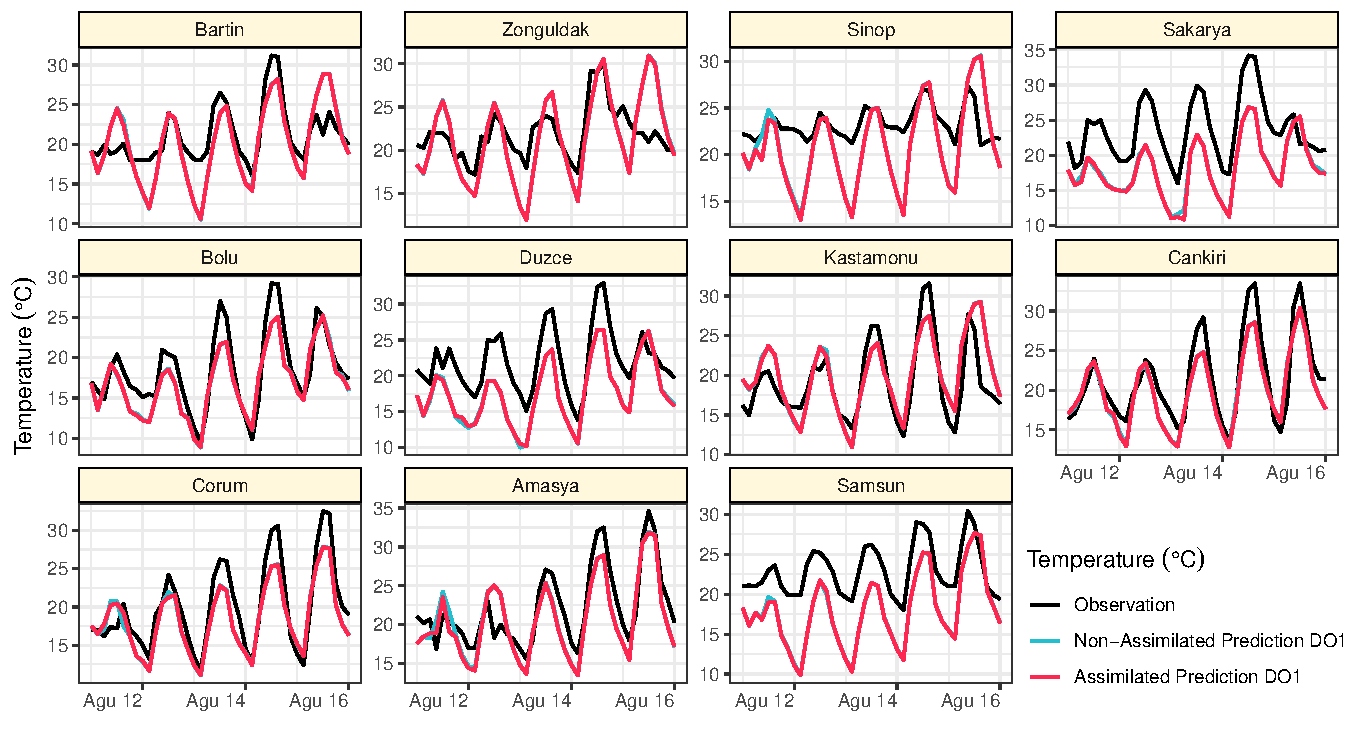
\includegraphics{WRF_pdf_files/figure-pdf/fig-do1-1.pdf}

}

\caption{\label{fig-do1}Comparison of predictions with observations for
each province in domain 1.}

\end{figure}

Figure~\ref{fig-sc1} is shown for scatterplot and heatmap of 3-hour
assimilated and non-assimilated predictions versus observations in
domain 1. \textbf{Red} and \textbf{blue} colors represent
\textbf{assimilated} and \textbf{non-assimilated} predictions,
respectively, while \textbf{black} line shows \textbf{fit} of
observations versus predictions.

According to the below plots, there is a clear linear relationship for
3-hour assimilated and non-assimilated predictions with observations in
domain 1.

\begin{Shaded}
\begin{Highlighting}[]
\NormalTok{plot1}\OtherTok{\textless{}{-}} 
\NormalTok{  new\_df\_list[[}\DecValTok{1}\NormalTok{]] }\SpecialCharTok{|\textgreater{}}        
    \FunctionTok{left\_join}\NormalTok{(new\_df\_list[[}\DecValTok{3}\NormalTok{]], }\AttributeTok{by =} \FunctionTok{c}\NormalTok{(}\StringTok{"Station"}\NormalTok{,}\StringTok{"dates"}\NormalTok{,}\StringTok{"observation"}\NormalTok{)) }\SpecialCharTok{|\textgreater{}} 
      \FunctionTok{pivot\_longer}\NormalTok{(}
        \AttributeTok{cols =} \SpecialCharTok{{-}}\FunctionTok{c}\NormalTok{(}\DecValTok{1}\NormalTok{,}\DecValTok{2}\NormalTok{,}\DecValTok{4}\NormalTok{),}
        \AttributeTok{names\_to =} \StringTok{"Pred.Type"}\NormalTok{,}
        \AttributeTok{values\_to =} \StringTok{"Prediction"}\NormalTok{,}
        \AttributeTok{values\_drop\_na =} \ConstantTok{FALSE}\NormalTok{) }\SpecialCharTok{|\textgreater{}}
\FunctionTok{ggplot}\NormalTok{(}\FunctionTok{aes}\NormalTok{(}\AttributeTok{x=}\NormalTok{ observation, }\AttributeTok{y=}\NormalTok{Prediction, }\AttributeTok{color=}\NormalTok{Pred.Type)) }\SpecialCharTok{+}   
  \FunctionTok{theme\_bw}\NormalTok{() }\SpecialCharTok{+}
  \FunctionTok{geom\_point}\NormalTok{(}\AttributeTok{size=}\DecValTok{2}\NormalTok{, }\AttributeTok{alpha=}\FloatTok{0.5}\NormalTok{) }\SpecialCharTok{+}   
  \FunctionTok{geom\_smooth}\NormalTok{(}\AttributeTok{color =}\StringTok{"black"}\NormalTok{, }\AttributeTok{se=}\ConstantTok{FALSE}\NormalTok{) }\SpecialCharTok{+}
  \FunctionTok{scale\_colour\_manual}\NormalTok{(}\AttributeTok{name=} \StringTok{" "}\NormalTok{, }
          \AttributeTok{values =} \FunctionTok{c}\NormalTok{(}\StringTok{\textquotesingle{}predict\_do1\_nas\textquotesingle{}} \OtherTok{=} \StringTok{"blue"}\NormalTok{,}
                     \StringTok{\textquotesingle{}predict\_do1\textquotesingle{}} \OtherTok{=} \StringTok{"\#fc2852"}\NormalTok{),}
          \AttributeTok{labels =} \FunctionTok{c}\NormalTok{(}\StringTok{\textquotesingle{}predict\_do1\_nas\textquotesingle{}} \OtherTok{=} \StringTok{\textquotesingle{}Non{-}Assimilated Prediction DO1\textquotesingle{}}\NormalTok{,}
                     \StringTok{\textquotesingle{}predict\_do1\textquotesingle{}} \OtherTok{=} \StringTok{\textquotesingle{}Assimilated Prediction DO1\textquotesingle{}}\NormalTok{)) }\SpecialCharTok{+}
  \FunctionTok{labs}\NormalTok{(}\AttributeTok{x=}\StringTok{"Observation"}\NormalTok{,}\AttributeTok{y=}\StringTok{"Prediction"}\NormalTok{) }\SpecialCharTok{+} \FunctionTok{theme}\NormalTok{(}\AttributeTok{legend.position =} \StringTok{"top"}\NormalTok{)}

\NormalTok{plot2}\OtherTok{\textless{}{-}} 
\NormalTok{  new\_df\_list[[}\DecValTok{1}\NormalTok{]] }\SpecialCharTok{|\textgreater{}}
    \FunctionTok{left\_join}\NormalTok{(new\_df\_list[[}\DecValTok{3}\NormalTok{]], }\AttributeTok{by =} \FunctionTok{c}\NormalTok{(}\StringTok{"Station"}\NormalTok{,}\StringTok{"dates"}\NormalTok{,}\StringTok{"observation"}\NormalTok{)) }\SpecialCharTok{|\textgreater{}}
      \FunctionTok{pivot\_longer}\NormalTok{(}
        \AttributeTok{cols =} \SpecialCharTok{{-}}\FunctionTok{c}\NormalTok{(}\DecValTok{1}\NormalTok{,}\DecValTok{2}\NormalTok{,}\DecValTok{4}\NormalTok{),}
        \AttributeTok{names\_to =} \StringTok{"Pred.Type"}\NormalTok{,}
        \AttributeTok{values\_to =} \StringTok{"Prediction"}\NormalTok{,}
        \AttributeTok{values\_drop\_na =} \ConstantTok{FALSE}\NormalTok{) }\SpecialCharTok{|\textgreater{}}
\FunctionTok{ggplot}\NormalTok{(}\FunctionTok{aes}\NormalTok{(}\AttributeTok{x=}\NormalTok{ observation, }\AttributeTok{y=}\NormalTok{Prediction, }\AttributeTok{fill=}\NormalTok{Pred.Type)) }\SpecialCharTok{+} 
  \FunctionTok{geom\_hex}\NormalTok{(}\AttributeTok{alpha=}\FloatTok{0.5}\NormalTok{) }\SpecialCharTok{+} \FunctionTok{theme\_bw}\NormalTok{() }\SpecialCharTok{+}
  \FunctionTok{scale\_fill\_manual}\NormalTok{(}\AttributeTok{name=} \StringTok{" "}\NormalTok{,}
      \AttributeTok{values =} \FunctionTok{c}\NormalTok{(}\StringTok{\textquotesingle{}predict\_do1\_nas\textquotesingle{}} \OtherTok{=} \StringTok{"blue"}\NormalTok{,}
                  \StringTok{\textquotesingle{}predict\_do1\textquotesingle{}} \OtherTok{=} \StringTok{"red"}\NormalTok{),}
      \AttributeTok{labels =} \FunctionTok{c}\NormalTok{(}\StringTok{\textquotesingle{}predict\_do1\_nas\textquotesingle{}} \OtherTok{=} \StringTok{\textquotesingle{}Non{-}Assimilated Prediction DO1\textquotesingle{}}\NormalTok{,}
                  \StringTok{\textquotesingle{}predict\_do1\textquotesingle{}} \OtherTok{=} \StringTok{\textquotesingle{}Assimilated Prediction DO1\textquotesingle{}}\NormalTok{)) }\SpecialCharTok{+}
  \FunctionTok{labs}\NormalTok{(}\AttributeTok{x=}\StringTok{"Observation"}\NormalTok{,}\AttributeTok{y=}\StringTok{"Prediction"}\NormalTok{) }\SpecialCharTok{+} \FunctionTok{theme}\NormalTok{(}\AttributeTok{legend.position =} \StringTok{"top"}\NormalTok{)}

\FunctionTok{ggarrange}\NormalTok{(plot1,plot2,}\AttributeTok{ncol=}\DecValTok{2}\NormalTok{ ,}\AttributeTok{nrow =} \DecValTok{1}\NormalTok{)}
\end{Highlighting}
\end{Shaded}

\begin{figure}[H]

{\centering 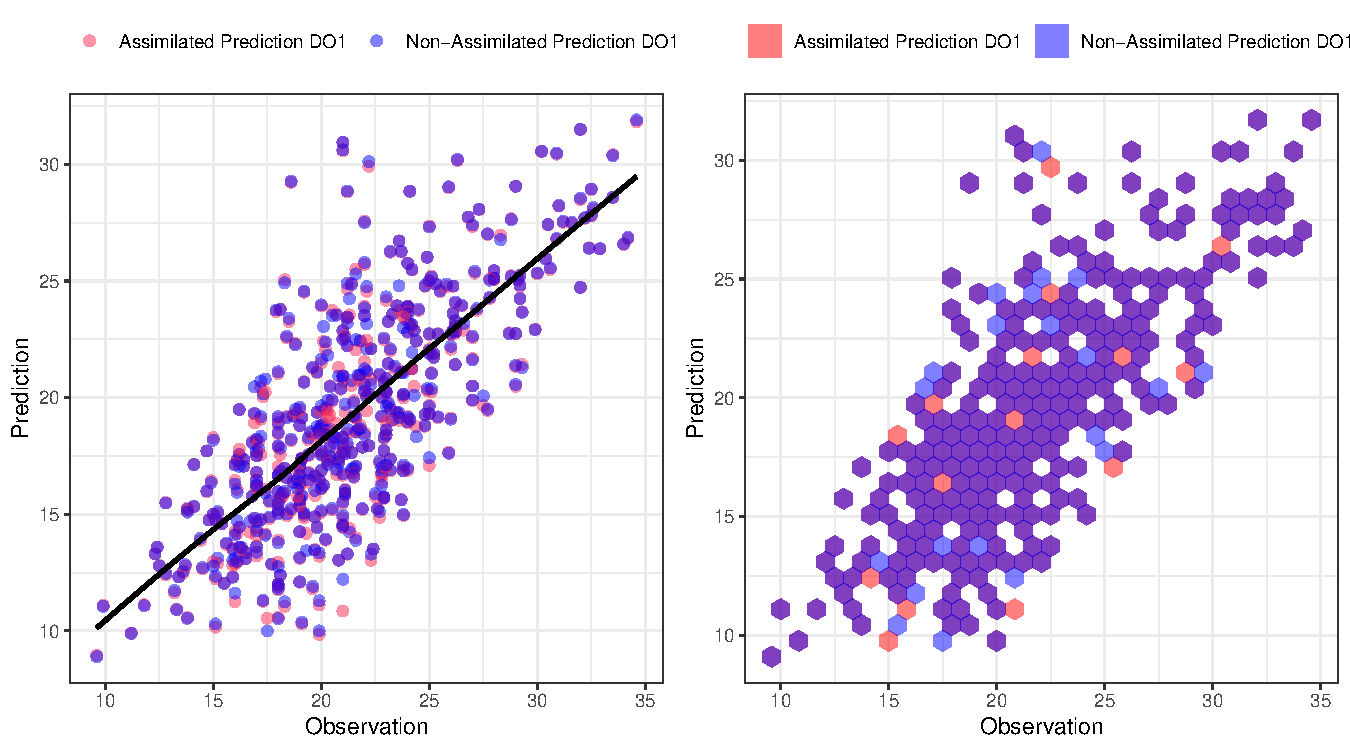
\includegraphics{WRF_pdf_files/figure-pdf/fig-sc1-1.pdf}

}

\caption{\label{fig-sc1}Scatterplot and heatmap of observations versus
predictions in domain 1.}

\end{figure}

Figure~\ref{fig-do2} is shown for comparison of hourly assimilated and
non-assimilated predictions with observations for each gauge
\emph{(province)} in domain 2. In this plot, each box represent
different provinces \emph{(gauges)}, \textbf{black} line shows
observations, \textbf{blue} and \textbf{red lines} are for
\textbf{assimilated} and \textbf{non-assimilated} predictions,
respectively.

The assimilated and non-assimilated predictions are looks like very
similar for also in domain 2. Hourly assimilated and non-assimilated
predictions are compatible with observations for Bartın, Zonguldak,
Kastamonu, Çorum and Samsun provinces but not remained provinces. It is
the fact that 3-hour predictions are looking better than hourly ones
even though domain 2 has finer resolution in both temporally and
spatially. Actually, this result also should be expected since increased
resolution may cause rise in error.

\begin{Shaded}
\begin{Highlighting}[]
\NormalTok{new\_df\_list[[}\DecValTok{2}\NormalTok{]] }\SpecialCharTok{|\textgreater{}}        
  \FunctionTok{left\_join}\NormalTok{(new\_df\_list[[}\DecValTok{4}\NormalTok{]], }\AttributeTok{by =} \FunctionTok{c}\NormalTok{(}\StringTok{"Station"}\NormalTok{,}\StringTok{"dates"}\NormalTok{,}\StringTok{"observation"}\NormalTok{)) }\SpecialCharTok{|\textgreater{}} 
    \FunctionTok{pivot\_longer}\NormalTok{(}
      \AttributeTok{cols =} \SpecialCharTok{{-}}\FunctionTok{c}\NormalTok{(}\DecValTok{1}\SpecialCharTok{:}\DecValTok{2}\NormalTok{),}
      \AttributeTok{names\_to =} \StringTok{"Temperature"}\NormalTok{,}
      \AttributeTok{values\_to =} \StringTok{"value"}\NormalTok{,}
      \AttributeTok{values\_drop\_na =} \ConstantTok{FALSE}\NormalTok{) }\SpecialCharTok{|\textgreater{}} 
  \FunctionTok{mutate}\NormalTok{(}\AttributeTok{Station =} \FunctionTok{factor}\NormalTok{(Station, }\AttributeTok{labels =}\NormalTok{ df\_gauges}\SpecialCharTok{$}\NormalTok{Province )) }\SpecialCharTok{|\textgreater{}}
  \FunctionTok{mutate}\NormalTok{(}\AttributeTok{Temperature =}  \FunctionTok{factor}\NormalTok{(Temperature, }
         \AttributeTok{levels=} \FunctionTok{c}\NormalTok{(}\StringTok{"observation"}\NormalTok{, }\StringTok{"predict\_do2\_nas"}\NormalTok{, }\StringTok{"predict\_do2"}\NormalTok{)) ) }\SpecialCharTok{|\textgreater{}}  
\FunctionTok{ggplot}\NormalTok{(}\FunctionTok{aes}\NormalTok{(}\AttributeTok{x=}\NormalTok{ dates, }\AttributeTok{y=}\NormalTok{value)) }\SpecialCharTok{+}   
  \FunctionTok{geom\_line}\NormalTok{(}\FunctionTok{aes}\NormalTok{(}\AttributeTok{colour =}\NormalTok{ Temperature), }\AttributeTok{size=}\FloatTok{0.7}\NormalTok{) }\SpecialCharTok{+}
  \FunctionTok{scale\_colour\_manual}\NormalTok{(}\AttributeTok{name=} \FunctionTok{expression}\NormalTok{(}\StringTok{"Temperature"}\SpecialCharTok{\textasciitilde{}}\NormalTok{(degree}\SpecialCharTok{*}\NormalTok{C)), }
          \AttributeTok{values =} \FunctionTok{c}\NormalTok{(}\StringTok{\textquotesingle{}observation\textquotesingle{}} \OtherTok{=} \StringTok{"black"}\NormalTok{,}
                     \StringTok{\textquotesingle{}predict\_do2\_nas\textquotesingle{}} \OtherTok{=} \StringTok{"\#fc2852"}\NormalTok{,}
                     \StringTok{\textquotesingle{}predict\_do2\textquotesingle{}} \OtherTok{=} \StringTok{"\#23bfce"}\NormalTok{),}
          \AttributeTok{labels =} \FunctionTok{c}\NormalTok{(}\StringTok{\textquotesingle{}observation\textquotesingle{}} \OtherTok{=} \StringTok{\textquotesingle{}Observation\textquotesingle{}}\NormalTok{,}
                     \StringTok{\textquotesingle{}predict\_do2\_nas\textquotesingle{}} \OtherTok{=} \StringTok{\textquotesingle{}Non{-}Assimilated Prediction DO2\textquotesingle{}}\NormalTok{,}
                     \StringTok{\textquotesingle{}predict\_do2\textquotesingle{}} \OtherTok{=} \StringTok{\textquotesingle{}Assimilated Prediction DO2\textquotesingle{}}\NormalTok{)) }\SpecialCharTok{+} 
  \FunctionTok{theme\_bw}\NormalTok{() }\SpecialCharTok{+} \FunctionTok{facet\_wrap}\NormalTok{(}\SpecialCharTok{\textasciitilde{}}\NormalTok{Station, }\AttributeTok{scales =} \StringTok{"free\_y"}\NormalTok{) }\SpecialCharTok{+} 
  \FunctionTok{labs}\NormalTok{(}\AttributeTok{x=}\StringTok{" "}\NormalTok{,}\AttributeTok{y=}\FunctionTok{expression}\NormalTok{(}\StringTok{"Temperature"}\SpecialCharTok{\textasciitilde{}}\NormalTok{(degree}\SpecialCharTok{*}\NormalTok{C))) }\SpecialCharTok{+} 
  \FunctionTok{theme}\NormalTok{(}\AttributeTok{axis.text.x =} \FunctionTok{element\_text}\NormalTok{(}\AttributeTok{angle =} \DecValTok{0}\NormalTok{, }\AttributeTok{hjust =} \DecValTok{1}\NormalTok{))  }\SpecialCharTok{+}
  \FunctionTok{theme}\NormalTok{(}\AttributeTok{legend.position =} \FunctionTok{c}\NormalTok{(.}\DecValTok{88}\NormalTok{, .}\DecValTok{1}\NormalTok{), }
        \AttributeTok{strip.background =} \FunctionTok{element\_rect}\NormalTok{(}\AttributeTok{colour=}\StringTok{"black"}\NormalTok{, }\AttributeTok{fill=}\StringTok{"cornsilk"}\NormalTok{))}
\end{Highlighting}
\end{Shaded}

\begin{figure}[H]

{\centering 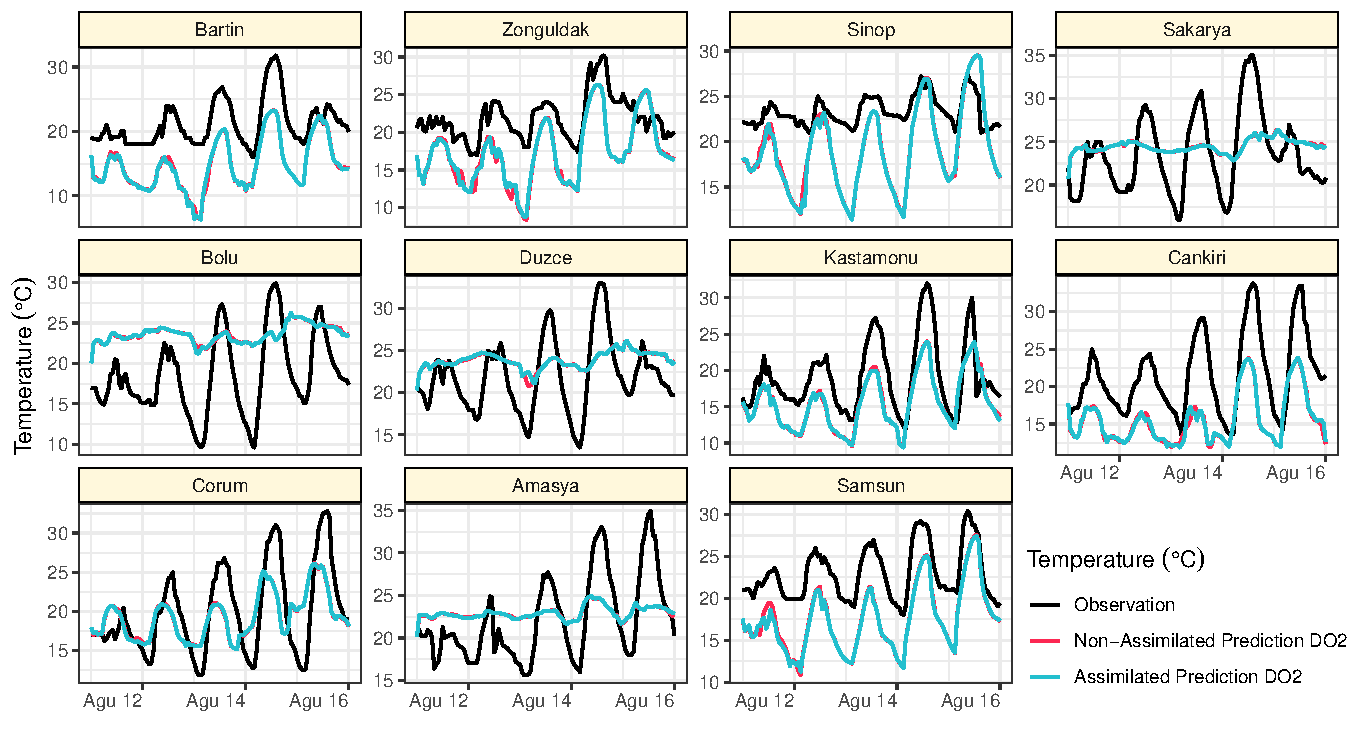
\includegraphics{WRF_pdf_files/figure-pdf/fig-do2-1.pdf}

}

\caption{\label{fig-do2}Comparison of predictions with observations for
each province in domain 2.}

\end{figure}

Figure~\ref{fig-sc2} is shown for scatterplot and heatmap of 1-hour
assimilated and non-assimilated predictions versus observations in
domain 2. \textbf{Blue} and \textbf{red} colors represent
\textbf{assimilated} and \textbf{non-assimilated} predictions,
respectively, while \textbf{black} line shows \textbf{fit} of
observations versus predictions.

According to the below plots, there is not a strong relationship between
hourly predictions and observations. We think that the reason of this
issue is that predictions are so smooth for Sakarya, Bolu, Duzce and
Amasya provinces. This situation causes two cluster on the scatterplot
and fluctuated fitting line.

\begin{Shaded}
\begin{Highlighting}[]
\NormalTok{plot3}\OtherTok{\textless{}{-}} 
\NormalTok{new\_df\_list[[}\DecValTok{2}\NormalTok{]] }\SpecialCharTok{|\textgreater{}}        
  \FunctionTok{left\_join}\NormalTok{(new\_df\_list[[}\DecValTok{4}\NormalTok{]], }\AttributeTok{by =} \FunctionTok{c}\NormalTok{(}\StringTok{"Station"}\NormalTok{,}\StringTok{"dates"}\NormalTok{,}\StringTok{"observation"}\NormalTok{)) }\SpecialCharTok{|\textgreater{}} 
    \FunctionTok{pivot\_longer}\NormalTok{(}
      \AttributeTok{cols =} \SpecialCharTok{{-}}\FunctionTok{c}\NormalTok{(}\DecValTok{1}\NormalTok{,}\DecValTok{2}\NormalTok{,}\DecValTok{4}\NormalTok{),}
      \AttributeTok{names\_to =} \StringTok{"Pred.Type"}\NormalTok{,}
      \AttributeTok{values\_to =} \StringTok{"Prediction"}\NormalTok{,}
      \AttributeTok{values\_drop\_na =} \ConstantTok{FALSE}\NormalTok{) }\SpecialCharTok{|\textgreater{}}
\FunctionTok{ggplot}\NormalTok{(}\FunctionTok{aes}\NormalTok{(}\AttributeTok{x=}\NormalTok{ observation, }\AttributeTok{y=}\NormalTok{Prediction, }\AttributeTok{color=}\NormalTok{Pred.Type)) }\SpecialCharTok{+}   
  \FunctionTok{theme\_bw}\NormalTok{() }\SpecialCharTok{+}
  \FunctionTok{geom\_point}\NormalTok{(}\AttributeTok{size=}\DecValTok{2}\NormalTok{, }\AttributeTok{alpha=}\FloatTok{0.5}\NormalTok{) }\SpecialCharTok{+}   
  \FunctionTok{geom\_smooth}\NormalTok{(}\AttributeTok{color =}\StringTok{"black"}\NormalTok{, }\AttributeTok{se=}\ConstantTok{FALSE}\NormalTok{) }\SpecialCharTok{+}
  \FunctionTok{scale\_colour\_manual}\NormalTok{(}\AttributeTok{name=} \StringTok{" "}\NormalTok{, }
    \AttributeTok{values =} \FunctionTok{c}\NormalTok{(}\StringTok{\textquotesingle{}predict\_do2\_nas\textquotesingle{}} \OtherTok{=} \StringTok{"\#fc2852"}\NormalTok{,}
               \StringTok{\textquotesingle{}predict\_do2\textquotesingle{}} \OtherTok{=} \StringTok{"blue"}\NormalTok{),}
    \AttributeTok{labels =} \FunctionTok{c}\NormalTok{(}\StringTok{\textquotesingle{}predict\_do2\_nas\textquotesingle{}} \OtherTok{=} \StringTok{\textquotesingle{}Non{-}Assimilated Prediction DO2\textquotesingle{}}\NormalTok{,}
               \StringTok{\textquotesingle{}predict\_do2\textquotesingle{}} \OtherTok{=} \StringTok{\textquotesingle{}Assimilated Prediction DO2\textquotesingle{}}\NormalTok{)) }\SpecialCharTok{+}
  \FunctionTok{labs}\NormalTok{(}\AttributeTok{x=}\StringTok{"Observation"}\NormalTok{,}\AttributeTok{y=}\StringTok{"Prediction"}\NormalTok{) }\SpecialCharTok{+} \FunctionTok{theme}\NormalTok{(}\AttributeTok{legend.position =} \StringTok{"top"}\NormalTok{)}

\NormalTok{plot4}\OtherTok{\textless{}{-}} 
\NormalTok{new\_df\_list[[}\DecValTok{2}\NormalTok{]] }\SpecialCharTok{|\textgreater{}}
  \FunctionTok{left\_join}\NormalTok{(new\_df\_list[[}\DecValTok{4}\NormalTok{]], }\AttributeTok{by =} \FunctionTok{c}\NormalTok{(}\StringTok{"Station"}\NormalTok{,}\StringTok{"dates"}\NormalTok{,}\StringTok{"observation"}\NormalTok{)) }\SpecialCharTok{|\textgreater{}}
    \FunctionTok{pivot\_longer}\NormalTok{(}
       \AttributeTok{cols =} \SpecialCharTok{{-}}\FunctionTok{c}\NormalTok{(}\DecValTok{1}\NormalTok{,}\DecValTok{2}\NormalTok{,}\DecValTok{4}\NormalTok{),}
       \AttributeTok{names\_to =} \StringTok{"Pred.Type"}\NormalTok{,}
       \AttributeTok{values\_to =} \StringTok{"Prediction"}\NormalTok{,}
       \AttributeTok{values\_drop\_na =} \ConstantTok{FALSE}\NormalTok{) }\SpecialCharTok{|\textgreater{}}
\FunctionTok{ggplot}\NormalTok{(}\FunctionTok{aes}\NormalTok{(}\AttributeTok{x=}\NormalTok{ observation, }\AttributeTok{y=}\NormalTok{Prediction, }\AttributeTok{fill=}\NormalTok{Pred.Type)) }\SpecialCharTok{+} 
  \FunctionTok{geom\_hex}\NormalTok{(}\AttributeTok{alpha=}\FloatTok{0.5}\NormalTok{) }\SpecialCharTok{+}     \FunctionTok{theme\_bw}\NormalTok{() }\SpecialCharTok{+}
  \FunctionTok{scale\_fill\_manual}\NormalTok{(}\AttributeTok{name=} \StringTok{" "}\NormalTok{,}
           \AttributeTok{values =} \FunctionTok{c}\NormalTok{(}\StringTok{\textquotesingle{}predict\_do2\_nas\textquotesingle{}} \OtherTok{=} \StringTok{"\#fc2852"}\NormalTok{,}
                      \StringTok{\textquotesingle{}predict\_do2\textquotesingle{}} \OtherTok{=} \StringTok{"blue"}\NormalTok{),}
           \AttributeTok{labels =} \FunctionTok{c}\NormalTok{(}\StringTok{\textquotesingle{}predict\_do2\_nas\textquotesingle{}} \OtherTok{=} \StringTok{\textquotesingle{}Non{-}Assimilated Prediction DO2\textquotesingle{}}\NormalTok{,}
                      \StringTok{\textquotesingle{}predict\_do2\textquotesingle{}} \OtherTok{=} \StringTok{\textquotesingle{}Assimilated Prediction DO2\textquotesingle{}}\NormalTok{)) }\SpecialCharTok{+}
  \FunctionTok{labs}\NormalTok{(}\AttributeTok{x=}\StringTok{"Observation"}\NormalTok{,}\AttributeTok{y=}\StringTok{"Prediction"}\NormalTok{) }\SpecialCharTok{+} \FunctionTok{theme}\NormalTok{(}\AttributeTok{legend.position =} \StringTok{"top"}\NormalTok{)}

\FunctionTok{ggarrange}\NormalTok{(plot3,plot4,}\AttributeTok{ncol=}\DecValTok{2}\NormalTok{ ,}\AttributeTok{nrow =} \DecValTok{1}\NormalTok{)}
\end{Highlighting}
\end{Shaded}

\begin{figure}[H]

{\centering 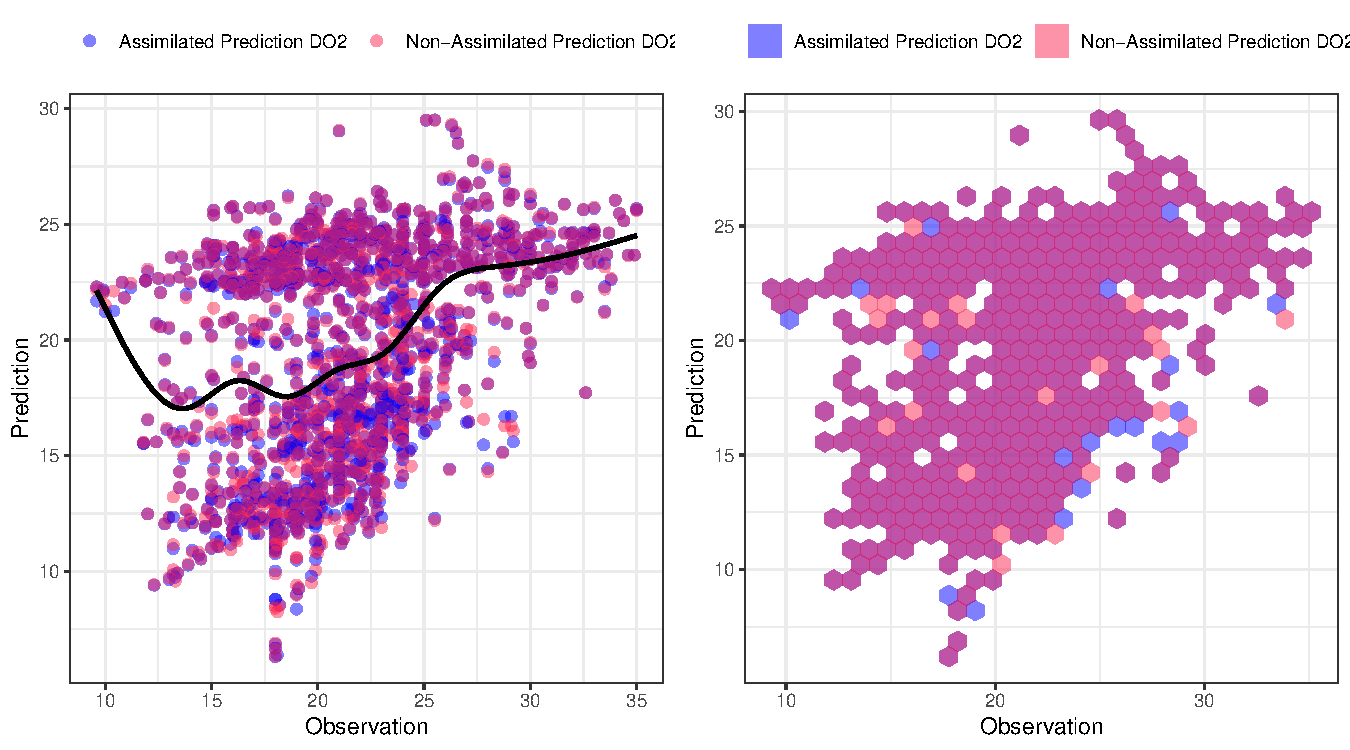
\includegraphics{WRF_pdf_files/figure-pdf/fig-sc2-1.pdf}

}

\caption{\label{fig-sc2}Scatterplot and heatmap of observations versus
predictions in domain 2.}

\end{figure}

Figure~\ref{fig-do1-2} is shown for comparison of three-hour assimilated
and non-assimilated predictions with observations for each gauge
\emph{(province)} in both two domains. In this plot, each box represent
different provinces \emph{(gauges)}, \textbf{black} line shows
observations, \textbf{pink} and \textbf{red} lines are for
\textbf{assimilated} and \textbf{non-assimilated} predictions in Domain
1, respectively. Additionally, \textbf{blue} and \textbf{lighter blue}
lines represent \textbf{assimilated} and \textbf{non-assimilated}
predictions in Domain 2, respectively.

This figure is providing us to compare all predictions and observations
in same plot for each province/gauge. The predictions in both two
domains are compatible except smoothed ones which are mentioned above.

\begin{Shaded}
\begin{Highlighting}[]
\NormalTok{new\_df\_list[[}\DecValTok{1}\NormalTok{]] }\SpecialCharTok{|\textgreater{}}        
  \FunctionTok{left\_join}\NormalTok{(new\_df\_list[[}\DecValTok{3}\NormalTok{]], }\AttributeTok{by =} \FunctionTok{c}\NormalTok{(}\StringTok{"Station"}\NormalTok{,}\StringTok{"dates"}\NormalTok{,}\StringTok{"observation"}\NormalTok{)) }\SpecialCharTok{|\textgreater{}} 
  \FunctionTok{left\_join}\NormalTok{(new\_df\_list[[}\DecValTok{2}\NormalTok{]], }\AttributeTok{by =} \FunctionTok{c}\NormalTok{(}\StringTok{"Station"}\NormalTok{,}\StringTok{"dates"}\NormalTok{,}\StringTok{"observation"}\NormalTok{)) }\SpecialCharTok{|\textgreater{}} 
  \FunctionTok{left\_join}\NormalTok{(new\_df\_list[[}\DecValTok{4}\NormalTok{]], }\AttributeTok{by =} \FunctionTok{c}\NormalTok{(}\StringTok{"Station"}\NormalTok{,}\StringTok{"dates"}\NormalTok{,}\StringTok{"observation"}\NormalTok{)) }\SpecialCharTok{|\textgreater{}} 
    \FunctionTok{pivot\_longer}\NormalTok{(}
      \AttributeTok{cols =} \SpecialCharTok{{-}}\FunctionTok{c}\NormalTok{(}\DecValTok{1}\NormalTok{,}\DecValTok{2}\NormalTok{),}
      \AttributeTok{names\_to =} \StringTok{"Temperature"}\NormalTok{,}
      \AttributeTok{values\_to =} \StringTok{"value"}\NormalTok{,}
      \AttributeTok{values\_drop\_na =} \ConstantTok{FALSE}\NormalTok{) }\SpecialCharTok{|\textgreater{}} 
  \FunctionTok{mutate}\NormalTok{(}\AttributeTok{Station =} \FunctionTok{factor}\NormalTok{(Station, }\AttributeTok{labels =}\NormalTok{ df\_gauges}\SpecialCharTok{$}\NormalTok{Province )) }\SpecialCharTok{|\textgreater{}}
  \FunctionTok{mutate}\NormalTok{(}\AttributeTok{Temperature =}  \FunctionTok{factor}\NormalTok{(Temperature, }
         \AttributeTok{levels=} \FunctionTok{c}\NormalTok{(}\StringTok{"observation"}\NormalTok{, }\StringTok{"predict\_do1"}\NormalTok{, }\StringTok{"predict\_do1\_nas"}\NormalTok{,}
                   \StringTok{"predict\_do2\_nas"}\NormalTok{, }\StringTok{"predict\_do2"}\NormalTok{)) ) }\SpecialCharTok{|\textgreater{}} 
\FunctionTok{ggplot}\NormalTok{(}\FunctionTok{aes}\NormalTok{(}\AttributeTok{x=}\NormalTok{ dates, }\AttributeTok{y=}\NormalTok{value)) }\SpecialCharTok{+}   
  \FunctionTok{geom\_line}\NormalTok{(}\FunctionTok{aes}\NormalTok{(}\AttributeTok{colour =}\NormalTok{ Temperature), }\AttributeTok{size=}\FloatTok{0.7}\NormalTok{) }\SpecialCharTok{+}
  \FunctionTok{scale\_colour\_manual}\NormalTok{(}\AttributeTok{name=} \FunctionTok{expression}\NormalTok{(}\StringTok{"Temperature"}\SpecialCharTok{\textasciitilde{}}\NormalTok{(degree}\SpecialCharTok{*}\NormalTok{C)), }
          \AttributeTok{values =} \FunctionTok{c}\NormalTok{(}\StringTok{\textquotesingle{}observation\textquotesingle{}} \OtherTok{=} \StringTok{"black"}\NormalTok{,}
                     \StringTok{\textquotesingle{}predict\_do1\_nas\textquotesingle{}} \OtherTok{=} \StringTok{"\#fc2852"}\NormalTok{,}
                     \StringTok{\textquotesingle{}predict\_do1\textquotesingle{}} \OtherTok{=} \StringTok{"\#fc95aa"}\NormalTok{,}
                     \StringTok{\textquotesingle{}predict\_do2\_nas\textquotesingle{}} \OtherTok{=} \StringTok{"\#23bfce"}\NormalTok{,}
                     \StringTok{\textquotesingle{}predict\_do2\textquotesingle{}} \OtherTok{=} \StringTok{"\#157882"}\NormalTok{),}
          \AttributeTok{labels =} \FunctionTok{c}\NormalTok{(}\StringTok{\textquotesingle{}observation\textquotesingle{}} \OtherTok{=} \StringTok{\textquotesingle{}Observation\textquotesingle{}}\NormalTok{,}
                     \StringTok{\textquotesingle{}predict\_do1\_nas\textquotesingle{}} \OtherTok{=} \StringTok{\textquotesingle{}Non{-}Assimilated Prediction DO1\textquotesingle{}}\NormalTok{,}
                     \StringTok{\textquotesingle{}predict\_do1\textquotesingle{}} \OtherTok{=} \StringTok{\textquotesingle{}Assimilated Prediction DO1\textquotesingle{}}\NormalTok{,}
                     \StringTok{\textquotesingle{}predict\_do2\_nas\textquotesingle{}} \OtherTok{=} \StringTok{\textquotesingle{}Non{-}Assimilated Prediction DO2\textquotesingle{}}\NormalTok{,}
                     \StringTok{\textquotesingle{}predict\_do2\textquotesingle{}} \OtherTok{=} \StringTok{\textquotesingle{}Assimilated Prediction DO2\textquotesingle{}}\NormalTok{)) }\SpecialCharTok{+}
  \FunctionTok{theme\_bw}\NormalTok{() }\SpecialCharTok{+} 
  \FunctionTok{facet\_wrap}\NormalTok{(}\SpecialCharTok{\textasciitilde{}}\NormalTok{Station, }\AttributeTok{scales =} \StringTok{"free\_y"}\NormalTok{) }\SpecialCharTok{+} 
  \FunctionTok{labs}\NormalTok{(}\AttributeTok{x=}\StringTok{" "}\NormalTok{,}\AttributeTok{y=}\FunctionTok{expression}\NormalTok{(}\StringTok{"Temperature"}\SpecialCharTok{\textasciitilde{}}\NormalTok{(degree}\SpecialCharTok{*}\NormalTok{C))) }\SpecialCharTok{+} 
  \FunctionTok{theme}\NormalTok{(}\AttributeTok{axis.text.x =} \FunctionTok{element\_text}\NormalTok{(}\AttributeTok{angle =} \DecValTok{0}\NormalTok{, }\AttributeTok{hjust =} \DecValTok{1}\NormalTok{))  }\SpecialCharTok{+}
  \FunctionTok{theme}\NormalTok{(}\AttributeTok{legend.position =} \FunctionTok{c}\NormalTok{(.}\DecValTok{88}\NormalTok{, .}\DecValTok{1}\NormalTok{), }
        \AttributeTok{strip.background =} \FunctionTok{element\_rect}\NormalTok{(}\AttributeTok{colour=}\StringTok{"black"}\NormalTok{, }\AttributeTok{fill=}\StringTok{"cornsilk"}\NormalTok{))}
\end{Highlighting}
\end{Shaded}

\begin{figure}[H]

{\centering 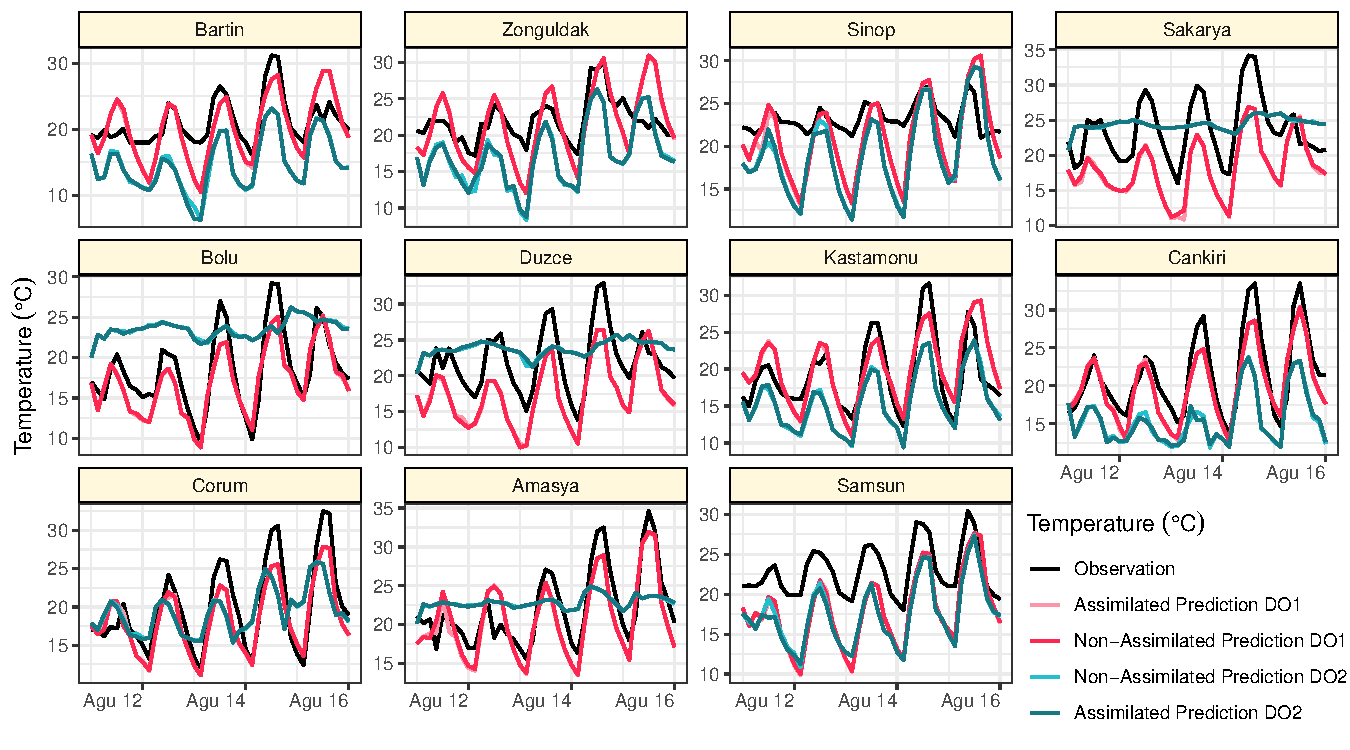
\includegraphics{WRF_pdf_files/figure-pdf/fig-do1-2-1.pdf}

}

\caption{\label{fig-do1-2}Comparison of predictions with observations
for each province in both two domains.}

\end{figure}

\hypertarget{error-analysis}{%
\subsection{Error Analysis}\label{error-analysis}}

This part calculates various error metrics, including bias, mean squared
error (MSE), root mean squared error (RMSE), normalized RMSE (NRMSE),
and correlation coefficients for the predictions. Table~\ref{tbl-stats}
shows the error statistics for both two domains with respect to complete
assimilated and non-assimilated predictions.

As an expected result, prediction errors in domain 2 are bigger than
domain 1 and correlation coefficient is also worse. Surprisingly,
assimilated prediction errors are not less than non-assimilated versions
when we compared each domain between among themselves. We think that
this situation is also caused smoothed predictions as mentioned
previously. Thus, errors for only Kastomunu province which has more
appropriate predictions in both domains is given below. Additionally, to
examine the opposite of this situation Duzce case is also given below.

\begin{Shaded}
\begin{Highlighting}[]
\CommentTok{\#BIAS}
\NormalTok{bias }\OtherTok{\textless{}{-}} \ControlFlowTok{function}\NormalTok{(x,y) \{}\FunctionTok{mean}\NormalTok{((x}\SpecialCharTok{{-}}\NormalTok{y), }\AttributeTok{na.rm =} \ConstantTok{TRUE}\NormalTok{)\}}
\CommentTok{\#MSE}
\NormalTok{mse}\OtherTok{\textless{}{-}} \ControlFlowTok{function}\NormalTok{(x,y) \{}\FunctionTok{mean}\NormalTok{((x}\SpecialCharTok{{-}}\NormalTok{y)}\SpecialCharTok{\^{}}\DecValTok{2}\NormalTok{, }\AttributeTok{na.rm =} \ConstantTok{TRUE}\NormalTok{)\}}
\CommentTok{\#RMSE}
\NormalTok{rmse}\OtherTok{\textless{}{-}} \ControlFlowTok{function}\NormalTok{(x,y) \{}\FunctionTok{sqrt}\NormalTok{( }\FunctionTok{mean}\NormalTok{( (x}\SpecialCharTok{{-}}\NormalTok{y)}\SpecialCharTok{\^{}}\DecValTok{2}\NormalTok{, }\AttributeTok{na.rm =} \ConstantTok{TRUE}\NormalTok{) )\}}
\CommentTok{\#NRMSE}
\NormalTok{nrmse}\OtherTok{\textless{}{-}} \ControlFlowTok{function}\NormalTok{(x,y)\{}\FunctionTok{sqrt}\NormalTok{( }\FunctionTok{mean}\NormalTok{((x}\SpecialCharTok{{-}}\NormalTok{y)}\SpecialCharTok{\^{}}\DecValTok{2}\NormalTok{, }\AttributeTok{na.rm =} \ConstantTok{TRUE}\NormalTok{) ) }\SpecialCharTok{/}\NormalTok{ (}\FunctionTok{max}\NormalTok{(x)}\SpecialCharTok{{-}}\FunctionTok{min}\NormalTok{(y))\}}


\CommentTok{\# domain1: new\_df\_list[[1]]; new\_df\_list[[3]]}
\CommentTok{\# domain2: new\_df\_list[[2]]; head(new\_df\_list[[4]])}

\NormalTok{error\_table}\OtherTok{\textless{}{-}} \FunctionTok{data.frame}\NormalTok{(}
                   \AttributeTok{Statistics =} \FunctionTok{c}\NormalTok{(}\StringTok{"BIAS"}\NormalTok{,}\StringTok{"MSE"}\NormalTok{,}\StringTok{"RMSE"}\NormalTok{,}\StringTok{"NRMSE"}\NormalTok{,}\StringTok{"COR.COEF"}\NormalTok{), }
                   \AttributeTok{Assim\_DO1 =} \DecValTok{1}\SpecialCharTok{:}\DecValTok{5}\NormalTok{, }
                   \AttributeTok{Assim\_DO2 =} \DecValTok{1}\SpecialCharTok{:}\DecValTok{5}\NormalTok{, }
                   \AttributeTok{Non\_Assim\_DO1 =} \DecValTok{1}\SpecialCharTok{:}\DecValTok{5}\NormalTok{,   }
                   \AttributeTok{Non\_Assim\_DO2 =} \DecValTok{1}\SpecialCharTok{:}\DecValTok{5}\NormalTok{)}


\ControlFlowTok{for}\NormalTok{ (i }\ControlFlowTok{in} \DecValTok{1}\SpecialCharTok{:}\DecValTok{4}\NormalTok{) \{}
\NormalTok{  error\_table[}\DecValTok{1}\NormalTok{,i}\SpecialCharTok{+}\DecValTok{1}\NormalTok{] }\OtherTok{\textless{}{-}} \FunctionTok{bias}\NormalTok{(}\FunctionTok{as.matrix}\NormalTok{(new\_df\_list[[i]][,}\DecValTok{4}\NormalTok{]), }
                           \FunctionTok{as.matrix}\NormalTok{(new\_df\_list[[i]][,}\DecValTok{3}\NormalTok{]))}
\NormalTok{  error\_table[}\DecValTok{2}\NormalTok{,i}\SpecialCharTok{+}\DecValTok{1}\NormalTok{] }\OtherTok{\textless{}{-}} \FunctionTok{mse}\NormalTok{(}\FunctionTok{as.matrix}\NormalTok{(new\_df\_list[[i]][,}\DecValTok{4}\NormalTok{]), }
                           \FunctionTok{as.matrix}\NormalTok{(new\_df\_list[[i]][,}\DecValTok{3}\NormalTok{]))}
\NormalTok{  error\_table[}\DecValTok{3}\NormalTok{,i}\SpecialCharTok{+}\DecValTok{1}\NormalTok{] }\OtherTok{\textless{}{-}} \FunctionTok{rmse}\NormalTok{(}\FunctionTok{as.matrix}\NormalTok{(new\_df\_list[[i]][,}\DecValTok{4}\NormalTok{]), }
                           \FunctionTok{as.matrix}\NormalTok{(new\_df\_list[[i]][,}\DecValTok{3}\NormalTok{]))}
\NormalTok{  error\_table[}\DecValTok{4}\NormalTok{,i}\SpecialCharTok{+}\DecValTok{1}\NormalTok{] }\OtherTok{\textless{}{-}} \FunctionTok{nrmse}\NormalTok{(}\FunctionTok{as.matrix}\NormalTok{(new\_df\_list[[i]][,}\DecValTok{4}\NormalTok{]), }
                           \FunctionTok{as.matrix}\NormalTok{(new\_df\_list[[i]][,}\DecValTok{3}\NormalTok{]))}
\NormalTok{  error\_table[}\DecValTok{5}\NormalTok{,i}\SpecialCharTok{+}\DecValTok{1}\NormalTok{] }\OtherTok{\textless{}{-}} \FunctionTok{cor}\NormalTok{(}\FunctionTok{as.matrix}\NormalTok{(new\_df\_list[[i]][,}\DecValTok{4}\NormalTok{]), }
                           \FunctionTok{as.matrix}\NormalTok{(new\_df\_list[[i]][,}\DecValTok{3}\NormalTok{]), }\AttributeTok{use=}\StringTok{\textquotesingle{}pairwise.complete.obs\textquotesingle{}}\NormalTok{)}
\NormalTok{               \}}

\NormalTok{error\_table[,}\DecValTok{2}\SpecialCharTok{:}\DecValTok{5}\NormalTok{]}\OtherTok{\textless{}{-}} \FunctionTok{round}\NormalTok{(error\_table[,}\DecValTok{2}\SpecialCharTok{:}\DecValTok{5}\NormalTok{],}\DecValTok{4}\NormalTok{)}
\NormalTok{error\_table }\SpecialCharTok{|\textgreater{}}  \FunctionTok{gt}\NormalTok{()}
\end{Highlighting}
\end{Shaded}

\hypertarget{tbl-stats}{}
\begin{longtable}{lrrrr}
\caption{\label{tbl-stats}Error statistics of entire predictions in each domain. }\tabularnewline

\toprule
Statistics & Assim\_DO1 & Assim\_DO2 & Non\_Assim\_DO1 & Non\_Assim\_DO2 \\ 
\midrule\addlinespace[2.5pt]
BIAS & 2.1705 & 2.0086 & 2.1191 & 1.9911 \\ 
MSE & 15.5098 & 30.5784 & 15.3419 & 30.4394 \\ 
RMSE & 3.9383 & 5.5298 & 3.9169 & 5.5172 \\ 
NRMSE & 0.1536 & 0.1927 & 0.1524 & 0.1924 \\ 
COR.COEF & 0.7477 & 0.3793 & 0.7466 & 0.3812 \\ 
\bottomrule
\end{longtable}

Table~\ref{tbl-kastamonu} shows the error statistics with respect to
assimilated and non-assimilated predictions for \textbf{Kastomonu}
province in both two domains.

When we investigate the results for only Kastomunu gauge/province
assimilated predictions have less errors slightly and better correlation
than non-assimilated ones in both two domains.

\begin{Shaded}
\begin{Highlighting}[]
\NormalTok{error\_table}\OtherTok{\textless{}{-}} \FunctionTok{data.frame}\NormalTok{(}
                   \AttributeTok{Statistics =} \FunctionTok{c}\NormalTok{(}\StringTok{"BIAS"}\NormalTok{,}\StringTok{"MSE"}\NormalTok{,}\StringTok{"RMSE"}\NormalTok{,}\StringTok{"NRMSE"}\NormalTok{,}\StringTok{"COR.COEF"}\NormalTok{), }
                   \AttributeTok{Assim\_DO1 =} \DecValTok{1}\SpecialCharTok{:}\DecValTok{5}\NormalTok{, }
                   \AttributeTok{Assim\_DO2 =} \DecValTok{1}\SpecialCharTok{:}\DecValTok{5}\NormalTok{, }
                   \AttributeTok{Non\_Assim\_DO1 =} \DecValTok{1}\SpecialCharTok{:}\DecValTok{5}\NormalTok{,   }
                   \AttributeTok{Non\_Assim\_DO2 =} \DecValTok{1}\SpecialCharTok{:}\DecValTok{5}\NormalTok{)}

\ControlFlowTok{for}\NormalTok{ (i }\ControlFlowTok{in} \DecValTok{1}\SpecialCharTok{:}\DecValTok{4}\NormalTok{) \{}
\NormalTok{  kastamonu}\OtherTok{\textless{}{-}} 
\NormalTok{      new\_df\_list[[i]] }\SpecialCharTok{|\textgreater{}} 
        \FunctionTok{mutate}\NormalTok{(}\AttributeTok{Station =} \FunctionTok{factor}\NormalTok{(Station, }\AttributeTok{labels =}\NormalTok{ df\_gauges}\SpecialCharTok{$}\NormalTok{Province )) }\SpecialCharTok{|\textgreater{}} 
        \FunctionTok{filter}\NormalTok{(Station }\SpecialCharTok{==} \StringTok{"Kastamonu"}\NormalTok{ )}
    
\NormalTok{  error\_table[}\DecValTok{1}\NormalTok{,i}\SpecialCharTok{+}\DecValTok{1}\NormalTok{] }\OtherTok{\textless{}{-}} \FunctionTok{bias}\NormalTok{(}\FunctionTok{as.matrix}\NormalTok{(kastamonu[,}\DecValTok{4}\NormalTok{]), }
                           \FunctionTok{as.matrix}\NormalTok{(kastamonu[,}\DecValTok{3}\NormalTok{]))}
\NormalTok{  error\_table[}\DecValTok{2}\NormalTok{,i}\SpecialCharTok{+}\DecValTok{1}\NormalTok{] }\OtherTok{\textless{}{-}} \FunctionTok{mse}\NormalTok{(}\FunctionTok{as.matrix}\NormalTok{(kastamonu[,}\DecValTok{4}\NormalTok{]), }
                           \FunctionTok{as.matrix}\NormalTok{(kastamonu[,}\DecValTok{3}\NormalTok{]))}
\NormalTok{  error\_table[}\DecValTok{3}\NormalTok{,i}\SpecialCharTok{+}\DecValTok{1}\NormalTok{] }\OtherTok{\textless{}{-}} \FunctionTok{rmse}\NormalTok{(}\FunctionTok{as.matrix}\NormalTok{(kastamonu[,}\DecValTok{4}\NormalTok{]), }
                           \FunctionTok{as.matrix}\NormalTok{(kastamonu[,}\DecValTok{3}\NormalTok{]))}
\NormalTok{  error\_table[}\DecValTok{4}\NormalTok{,i}\SpecialCharTok{+}\DecValTok{1}\NormalTok{] }\OtherTok{\textless{}{-}} \FunctionTok{nrmse}\NormalTok{(}\FunctionTok{as.matrix}\NormalTok{(kastamonu[,}\DecValTok{4}\NormalTok{]), }
                           \FunctionTok{as.matrix}\NormalTok{(kastamonu[,}\DecValTok{3}\NormalTok{]))}
\NormalTok{  error\_table[}\DecValTok{5}\NormalTok{,i}\SpecialCharTok{+}\DecValTok{1}\NormalTok{] }\OtherTok{\textless{}{-}} \FunctionTok{cor}\NormalTok{(}\FunctionTok{as.matrix}\NormalTok{(kastamonu[,}\DecValTok{4}\NormalTok{]), }
                           \FunctionTok{as.matrix}\NormalTok{(kastamonu[,}\DecValTok{3}\NormalTok{]), }\AttributeTok{use=}\StringTok{\textquotesingle{}pairwise.complete.obs\textquotesingle{}}\NormalTok{)}
\NormalTok{               \}}

\NormalTok{error\_table[,}\DecValTok{2}\SpecialCharTok{:}\DecValTok{5}\NormalTok{]}\OtherTok{\textless{}{-}} \FunctionTok{round}\NormalTok{(error\_table[,}\DecValTok{2}\SpecialCharTok{:}\DecValTok{5}\NormalTok{],}\DecValTok{4}\NormalTok{)}
\NormalTok{error\_table }\SpecialCharTok{|\textgreater{}}  \FunctionTok{gt}\NormalTok{()}
\end{Highlighting}
\end{Shaded}

\hypertarget{tbl-kastamonu}{}
\begin{longtable}{lrrrr}
\caption{\label{tbl-kastamonu}Error statistics of predictions for Kastomonu province in each domain. }\tabularnewline

\toprule
Statistics & Assim\_DO1 & Assim\_DO2 & Non\_Assim\_DO1 & Non\_Assim\_DO2 \\ 
\midrule\addlinespace[2.5pt]
BIAS & -0.7900 & 3.5949 & -0.8210 & 3.5408 \\ 
MSE & 9.2272 & 20.2453 & 9.2425 & 19.9165 \\ 
RMSE & 3.0376 & 4.4995 & 3.0401 & 4.4628 \\ 
NRMSE & 0.1469 & 0.1991 & 0.1469 & 0.1976 \\ 
COR.COEF & 0.8009 & 0.8327 & 0.8026 & 0.8304 \\ 
\bottomrule
\end{longtable}

Table~\ref{tbl-duzce} shows the error statistics with respect to
assimilated and non-assimilated predictions for \textbf{Duzce} province
in both two domains. In this example, errors are bigger in assimilated
versions and correlation coefficients smaller in domain 2.

\hypertarget{tbl-duzce}{}
\begin{longtable}{lrrrr}
\caption{\label{tbl-duzce}Error statistics of predictions for Duzce province in each domain. }\tabularnewline

\toprule
Statistics & Assim\_DO1 & Assim\_DO2 & Non\_Assim\_DO1 & Non\_Assim\_DO2 \\ 
\midrule\addlinespace[2.5pt]
BIAS & 4.3474 & -1.9797 & 4.3616 & -1.9523 \\ 
MSE & 24.4499 & 20.1177 & 24.7878 & 19.6618 \\ 
RMSE & 4.9447 & 4.4853 & 4.9787 & 4.4342 \\ 
NRMSE & 0.2174 & 0.3537 & 0.2174 & 0.3497 \\ 
COR.COEF & 0.8513 & 0.3535 & 0.8473 & 0.3886 \\ 
\bottomrule
\end{longtable}

\hypertarget{conclusion}{%
\section{Conclusion}\label{conclusion}}

In summary, the integration of the WRF model with data assimilation
techniques has proven to be a valuable tool for advancing our
understanding of regional weather patterns. The outcomes of this study
have practical applications in operational forecasting, research
endeavors, and emergency response, contributing to the broader field of
atmospheric science. These steps collectively demonstrate a
comprehensive workflow for importing, processing, and analyzing
meteorological data, including visualization and error analysis.


\printbibliography


\end{document}
